\documentclass[11pt,a4paper]{article}

%\usepackage[square]{natbib}
\usepackage[utf8]{inputenc}
\usepackage[czech]{babel}
\usepackage[T1]{fontenc}      % T1 kodovani fontu pro babel cestinu

\usepackage[unicode, colorlinks=true, citecolor=blue]{hyperref}

%\usepackage[T1]{fontenc}
%\usepackage{uarial}
%\renewcommand{\familydefault}{\sfdefault}
%\renewcommand{\rmdefault}{\sfdefault}
%\usepackage{sfmath}
%\usepackage{sansmath}

\usepackage{amsfonts,amsmath}
\usepackage{etoolbox}
\usepackage{graphicx}
\usepackage[unicode]{hyperref}
\usepackage{multirow}
\usepackage{titlesec}
\setcounter{secnumdepth}{3}
\usepackage{float}
\usepackage{caption}
\usepackage{subcaption}
\usepackage{setspace}
\usepackage{geometry}
\usepackage{calc}
\usepackage{booktabs}


\geometry{verbose,
          tmargin=4cm,
          bmargin=3cm,
          lmargin=2.5cm,
          rmargin=2.5cm,
          footskip=24pt}
% \newlength\mytopmargin
% \newsavebox{\headbox}\savebox{\headbox}{
%   \begin{flushleft}                           
%   
\includegraphics[width=2cm]{logo_TACR_zakl.pdf} 
%   \end{flushleft}}
% \setlength{\mytopmargin}{\totalheightof{\usebox{\headbox}}+2cm}
% \geometry{verbose,
%           tmargin=\mytopmargin,
%           headheight=1.1\mytopmargin}
% \usepackage{fancyhdr}
% \fancyhf{}
% \fancyhead[C]{\usebox\headbox}
% \renewcommand{\headrulewidth}{0pt}
\usepackage{fancyhdr}
\pagestyle{fancy}
\renewcommand{\headrulewidth}{0pt}
\fancyhead[L]{\begin{picture}(0,0) 
\put(0,0){
\includegraphics[width=2cm]{logo_TACR_zakl.pdf}} 
\end{picture}}% empty left


% \usepackage{fancyhdr}
% %\pagestyle{fancy}
% \fancyhead{
% %     \begin{picture}(0,0)
% %         \put(-20,-10)
% %     \end{picture}
%     {
\includegraphics[width=2cm]{logo_TACR_zakl.pdf}}
%     \vbox{
%       Technologická agentura\\
%       České republiky
%     }
%     }
% \rhead{}    
% \cfoot{}
% \rfoot{\thepage}
% \renewcommand{\headrulewidth}{0pt}

\newcommand{\obraz}[1]{(viz obr. \ref{#1})}
\newcommand{\tabul}[1]{(viz tab. \ref{#1})}
\newcommand{\pozn}[1]{(viz odst. \ref{#1})}


\usepackage{tikz}

% macro for units.
\def\UNIT#1#2{\ifstrempty{#2}{}{%
\ifstrequal{#2}{1}{\mathrm{#1}}{\mathrm{#1}^{#2}}%
}}
\def\units#1#2#3{\ifstrempty{#1#2#3}{$[-]$}{$[ \UNIT{kg}{#1}\UNIT{m}{#2}\UNIT{s}{#3} ]$}} %with brackets
\def\unitss#1#2#3{\ifstrempty{#1#2#3}{$-$}{$ \UNIT{kg}{#1}\UNIT{m}{#2}\UNIT{s}{#3} $}}    %without brackets

%macro for hyperlinks (dummy)
\def\hyperA#1#2{#2}
  


% ***************************************** SYMBOLS
\def\abs#1{\lvert#1\rvert}
\def\argdot{{\hspace{0.18em}\cdot\hspace{0.18em}}}
\def\bb{\vc b}
\def\d{\mathrm{d}}
\def\D{{\tn D}}
\def\div{\operatorname{div}}
\def\grad{\nabla}
\def\jmp#1{[#1]}
\def\n{\vc n}
\def\nn{\vc n}
\def\prtl{\partial}
\def\R{\mathbb R}
\def\Real{\mathbb R}
\def\sc#1#2{\left(#1,#2\right)}
\def\th{\vartheta}
\def\tn#1{{\mathbb{#1}}}    % tensor
\def\vc#1{\mathbf{\boldsymbol{#1}}}     % vector
\def \E{{\mathsf E}}
\def\avg#1{\langle#1\rangle}
\def\var#1{\llangle#1\rrangle}
\def\Var{\mathop{\rm Var}}
\def\Cov{\mathop{\rm Cov}}
%\def\log{\mathop{\rm log}}
\def\abs#1{|#1|}

\def\vl{{\vc\lambda}}
\def\estvl{{\vc{\hat\lambda}}}
\def\estrho{\hat\rho}
\def\vmu{\vc\mu}
\def\estvmu{{\vc{\hat\mu}}}
\def\vphi{\vc\phi}

\newcommand{\jb}[1]{{\color{violet} JB: #1}}
\newcommand{\sy}[1]{{\color{blue} SS: #1}}
\newenvironment{old}{%
    \leavevmode\color{gray}\ignorespaces%
}{%
}%
%***************************************************************************



%TODO:
% články Bayes do referencí
% sjednotit Obr obraze
% update od Jakuba

\begin{document}
\begin{onehalfspacing} 

%\ULCornerWallPaper{1}{\includegraphics{TACR_logo.png}}
%\LLCornerWallPaper{1}{bar}
%\lipsum[1-3]

\begin{titlepage}
    
\includegraphics[width=2cm]{logo_TACR_zakl.pdf}

    \vspace{6cm}
    {\centering	
      {\scshape\bf\huge Odborná zpráva - \\
      řešení projektu Endorse v roce 2020\par}
    }
	
    \vspace{3cm}	
    {\LARGE
      {\noindent Číslo projektu:  TK02010118
        {\bfseries }\par}
      \vspace{2ex}
      {\noindent Název projektu: \\
        {\bfseries Predikce vlastností EDZ s vlivem na bezpečnost a spolehlivost
         hlubinného úložiště radioaktivního odpadu.} \par}
      \vspace{2ex}
      {\noindent Předkládá: \\
      \-\hspace{2ex} organizace: {\bfseries Technická univerzita v Liberci}\\
      \-\hspace{2ex} řešitel: {\bfseries doc. Mgr. Jan Březina, Ph.D.}\\
      \-\hspace{2ex} organizace: {\bfseries Ústav Geoniky}\\
      \-\hspace{2ex} spoluřešitel: {\bfseries prof. RNDr. Radim Blaheta CSc.}\par}

    }  
    \vfill
% Bottom of the page
\end{titlepage}

%\setcounter{page}{4}


\section{Úvod}
Projekt je řešen od 07/2019, tato zpráva shrnuje postup prací za rok 2020, což byl druhý rok řešení projektu. Řešení projektu bylo významně poznamenáno pandemií COVID-19 jednak sníženou kapacitou na obou pracovištích z důvodu přechodu na online vzdělávání, ale zejména pak v závěru roku vážným onemocněním spoluřešitele, prof. R. Blahety. Vzhledem k tomu, že není v tuto chvíli možné odhadnout délku nepřítomnosti spoluřešitele, lze očekávat, že tato situace bohužel ovlivní řešení projektu i v příštím roce. 


V roce 2020 byly dle harmonogramu projektu řešeny
aktivity:
\begin{itemize}
\item Definice vstupních dat a indikátorů bezpečnostních funkcí EDZ. (07/2019 - 07/2020)

\item Vývoj modelu proudění a mechaniky na smíšených sítích (07/2019 - 12/2020)

\item Matematické modely EDZ a související inverzní úlohy (1/2020 - 6/2021)

\item Knihovny pro stochastické přímé a inverzní metody (07/2019 - 12/2021)
\end{itemize}

 První aktivita, kapitola \ref{sec:indikatory}, byla zakončena milníkem v podobě rešeršní zprávy (v příloze). 

Milník druhé aktivity, kapitola \ref{sec:smisene_site} byl splněn dle rozsahu definovaného v harmonogramu.
Dle plánu byl implementován hydro-mechanický model s diskrétními puklinami. 
Pro správnou predikci hydraulické vodivosti však bude potřeba složitější model kontatků a tření na puklinách. V tomto směru bude probíhat další vývoj v rámci ostatních aktivit. 

Řešení třetí aktivity, kapitola \ref{sec:hm_modely}, se mírně zpozdilo kvůli sníženým pracovním kapacitám. Během roku se teprve upřesňovala její přesná náplň Tým TUL
se proto zatím věnoval s předstihem vývoji transportního modelu. Tým ÚGN otestoval 
použití existujícího plastického modelu a aplikaci Bayesovských metod na složitější hydro-mechanickou úlohu.

V rámci poslední aktivity, kapitola \ref{sec:stochastic}, byla dokončena další verze knihovny MLMC (multilevel Monte Carlo) pro stochastické výpočty a byly testovány pokročilejší metody rekonstrukce hustoty 
pravděpodobnosti. Vyvinuté metamodely (surogate) akceleraci Bayesovské inverze byly testovány na hydro-mechanických úlohách.

S předstihem byly sestaveny modely transportu, kapitola \ref{sec:transport}. Jednak zjednodušený model transportu geobariérou a zejména model transportu v EDZ s reálnou geometrií úložiště a vlivem náhodných geologických zlomů.
 

\section[Definice indikátorů bezpečnostních funkcí EDZ.]{Definice vstupních dat 
a indikátorů bezpečnostních funkcí~EDZ.}
\label{sec:indikatory}
{\it Období aktivity:}  07/2019 - 07/2020

\subsection{Popis aktivity dle přihlášky projektu}
{\it V úzké spolupráci s aplikačním garantem budou navrženy indikátory bezpečnosti pro EDZ v okolí úložiště. Indikátory budou
definovány buďto jako přímo měřitelné veličiny nebo jako veličiny odvozené od stavových veličin relevantních procesů (mechanika,
proudění, transport). Další řešení projektu pak bude zaměřeno na predikci těchto indikátorů pomocí vhodných modelů příslušných
procesů. Indikátory budou chápány jako náhodné veličiny
vzhledem k nejistotám v parametrech modelů a budou predikovány jejich hustoty pravděpodobnosti. Pro určení klíčových parametrů
zamýšlených modelů bude provedena rešerše dostupných apriorních dat (zejména dat pro Task G projektu Decovalex a data z
podzemní laboratoře Bukov). Dále bude ve spolupráci s aplikačním garantem sestaven přehled geofyzikálních měření aplikovatelných
v prostorách úložiště a bude odhadnuta jejich citlivost vůči parametrům modelů a finanční náročnost.}


\subsection{Řešení}
Na základě konzultací s aplikačním garantem byla navržena definice indikátorů bezpečnosti EDZ. Indikátory jsou 
odvozeny od výsledků modelu popisujícího proudění a transport v okolí jednoho úložného vrtu. Je popsán mechanický model 
 na škále průměru úložného vrtu a jsou představeny různé varianty konstitutivních vztahů pro popis vzniku EDZ. 
 Další kapitola je věnována empirickým vztahům pro závislost vodivosti a porozity na napětí a je představen možný
 víceškálový model, který by mohl umožnit přenos parametrů změřených v laboratorním měřítku na větší škály.
 V předposlední kapitole je uvedena rešerše měřících metod pro charakterizaci vlastností EDZ a v závěrečné kapitole je 
 popsán návrh validační úlohy pro modely vyvíjené v rámci projektu s využitím existujících zahraničních dat
 a jsou stručně nastíněny možnosti realizace validačního experimentu na PVP Bukov. 


\section{Vývoj modelu proudění a mechaniky na smíšených sítích}
\label{sec:smisene_site}
{\it Období aktivity:}  07/2019 - 12/2020


\subsection{Popis aktivity dle přihlášky projektu}
{ \it
Cílem aktivity je vývoj výpočetních kódů pro modely proudění a mechaniky v EDZ. Pro efektivní implementaci různých vazeb mezi
procesy bude existující simulátor Flow123d významně upraven s využitím knihovny FEniCS, to zahrnuje též implementaci podpory
smíšených sítí do knihovny FEniCS. V SW Flow123d budou dále implementovány modely proudění a mechaniky na smíšených sítích s
předpokladem malých deformací na puklinách.
Bude vyvinut model pro sdružené hydro-mechanické (HM) úlohy založený na iteračním přístupu a vhodném předpodmínění.
Budou vyvinuty modely mechaniky s explicitním popisem puklin založené na SW GEM a PERMON. V první fázi půjde o mechanický
model na smíšených sítích s pružným chováním matrice a s kontaktní formulací na trhlinách. Nerovnostní podmínka nepronikání na
trhlinách bude řešena zavedením Lagrangeových multiplikátorů.}

Aktivita má být zakončena milníkem: \uv{Modely proudění a mechaniky na smíšených sítích} zahrnujícím~modely pro testování různých způsobů popisu proudění a mechaniky rozpukaného porézního média. Zejména bylo plánováno následující rozšíření existujících simulátorů:
\begin{itemize}
\item Simulátor Flow123d s podporou pro pro sdružené hydro-mechanické úlohy na smíšených sítích.
\item Simulátor PERMON pro mechanický model na smíšených sítích s možností externího vstupu pórového tlaku a teplotní změny.
\end{itemize}

Lze konstatovat, že milník byl dle plánovaného rozsahu splněn což je demonstrováno níže na testovacích úlohách. Na základě další rešerše však předpokládáme 
nutnost použít pro realizaci víceškálového přístupu složitější model nelineárních procesů na puklinách proto bude jeho vývoj pokračovat během roku 2021. Nicméně cílů projektu lze dosáhnout i s použitím konzervativnějších modelů.


\subsection{Poroelastický modul ve Flow123d (TUL)}
V roce 2020 byl dokončen matematický model poroelasticity na smíšených sítí včetně jeho existenční analýzy.
Byla odvozena optimální hodnota relaxačního parametru iteračního schématu \uv{fixed-stress splitting} a dokázána konvergence tohoto schématu.
Výsledky byly sepsány a zaslány k publikaci v recenzovaném časopise \cite{brezina_stebel_preprint}.
Teoretické výsledky se promítly do implementace SW Flow123d, kde došlo k urychlení konvergence HM modelu díky vylepšené 
volbě relaxačního parametru a opravě chyby při výpočtu polí předávaných mezi řešičem proudění a mechaniky.
Simulátor Flow123d tak nyní umožňuje řešení 3d úloh lineární poroelasticity s diskrétní reprezentací puklin.

Pro demonstraci hydro-mechanického modelu ve Flow123d byla zvolena 2D úloha s 2 puklinami:
Pukliny mají 1000krát vyšší hydraulickou vodivost a 1000krát nižší Youngův modul než okolní prostředí, takto zvolené parametry řádově odpovídají změnám uvedených parametrů v EDZ oproti hodnotám v intaktní hornině.
Skrz pukliny je do oblasti vtláčena tekutina, viz obr. \ref{fig:hm_bc} s popisem okrajových podmínek.
Na obrázku \ref{fig:hm_results} je pak zobrazeno pole tlaku a posunutí.
Vzhledem k různým rozevřením puklin je deformace větší v okolí pukliny s větším rozevřením.
\begin{figure}
    \centering
    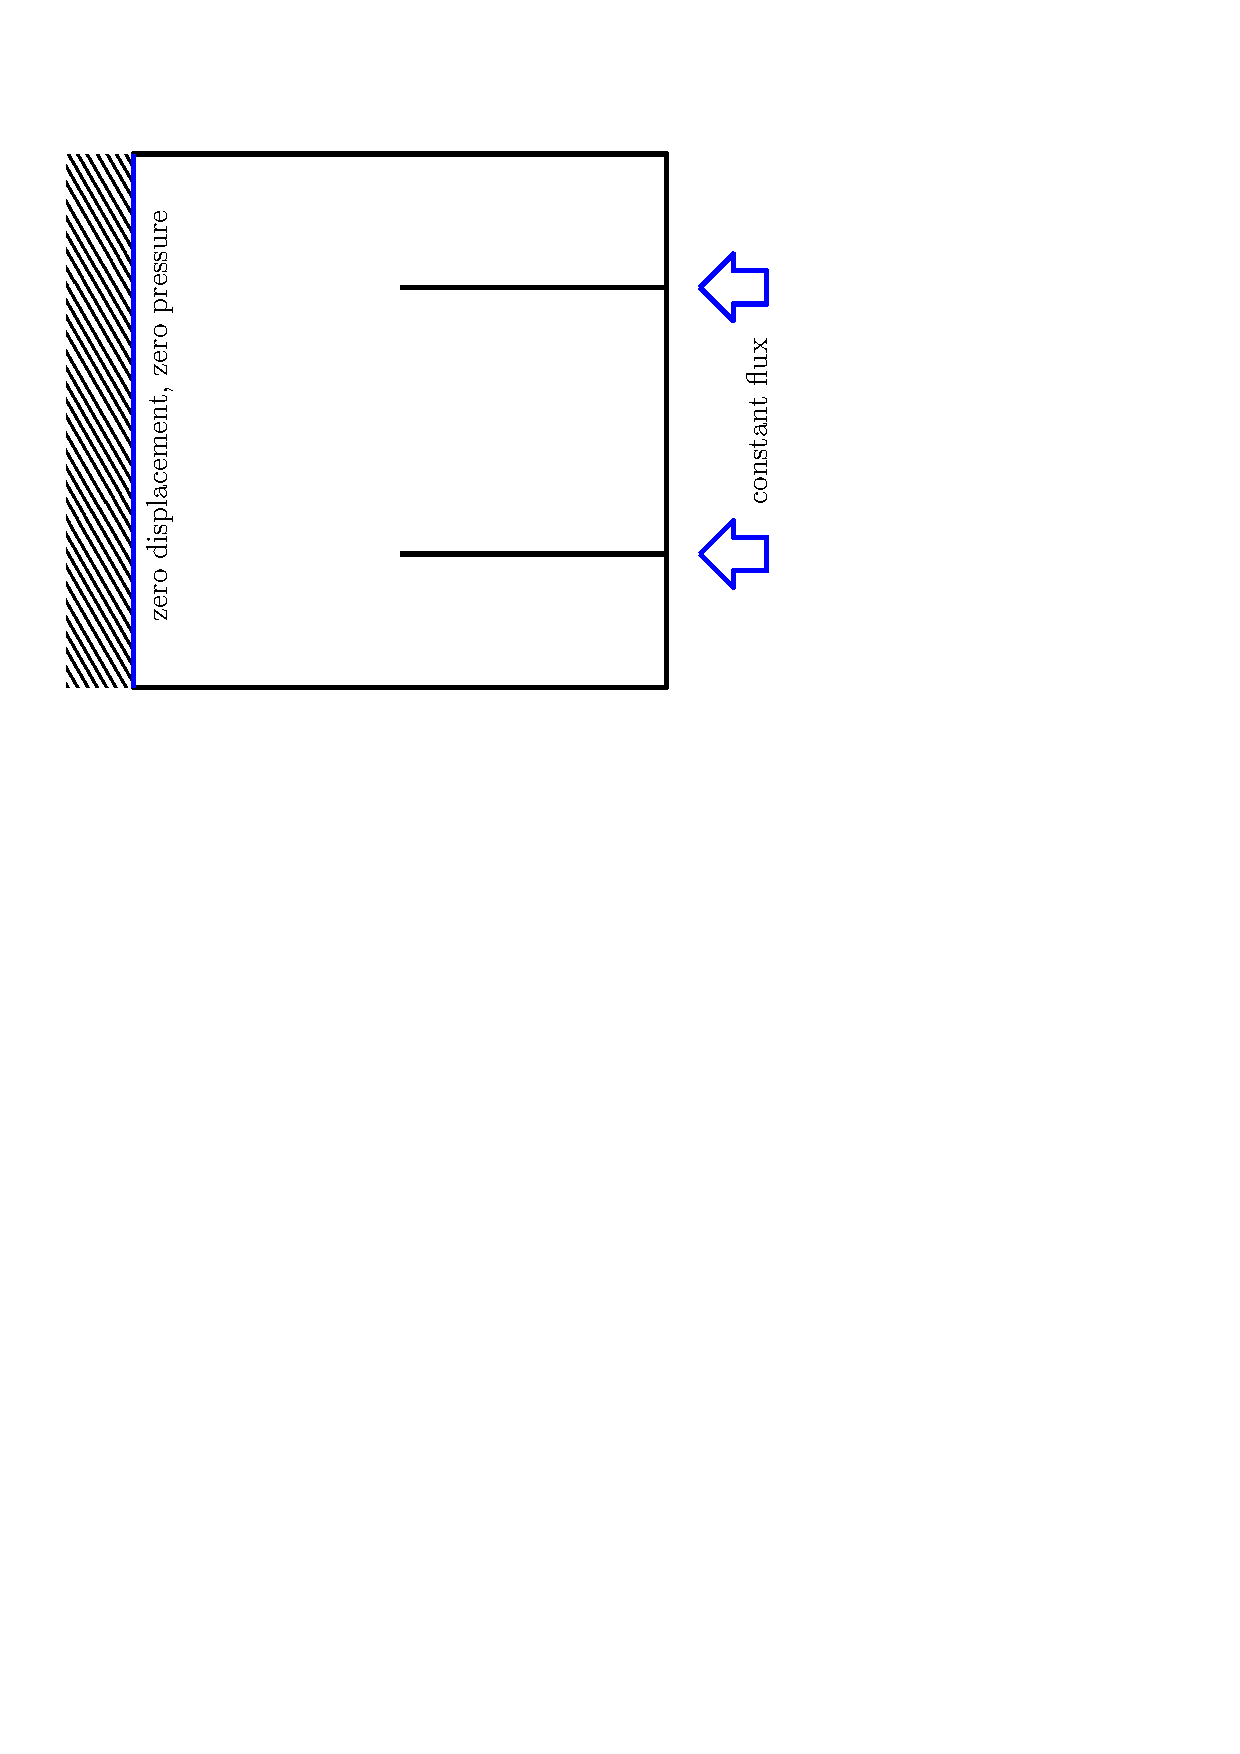
\includegraphics[width=0.5\textwidth]{graphics/obr_stebel/01_inject_bc.pdf}
    \caption{Demonstrační HM úloha: okrajové podmínky.}
    \label{fig:hm_bc}
\end{figure}

\begin{figure}
    \centering
    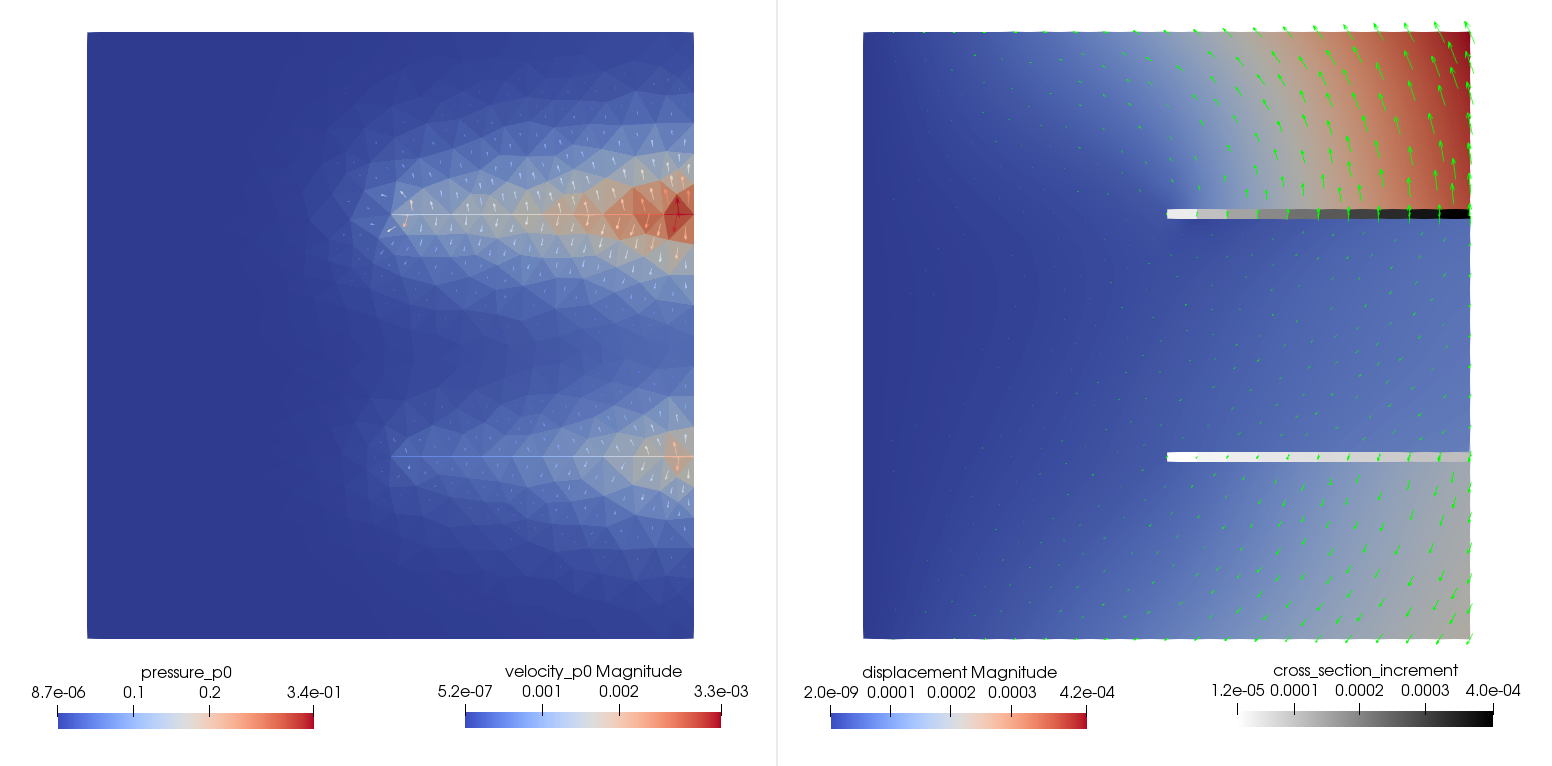
\includegraphics[width=\textwidth]{graphics/obr_stebel/01_inject.png}
    \caption{Demonstrační úloha: Vlevo pole tlaku a rychlosti, vpravo posunutí a rozevření puklin vlivem vtláčení.}
    \label{fig:hm_results}
\end{figure}


V souvislosti s řešením modelů EDZ v další fázi projektu byla studována možnost zahrnutí nelineárních 
interakcí na puklinách, zejména kontaktních podmínek (nepronikání), podmínek Coulombova tření a podmínek rozevírání vlivem smykového posunu.
Tyto podmínky mají významný vliv na hodnotu hydraulické vodivosti homogenizovaného média \cite{min_2004}.
Model s kontaktem byl výpočetně testován v prostředí FEniCS. V první fázi byl implementován s použitím primární formulace 
a Lagrangeova multiplikátoru. Tato formulace se ukázala nevyhovující jednak kvůli citlivosti na volbu diskretizačních 
prostorů a dále kvůli nestabilitě řešiče vzniklé optimalizační úlohy. Proto byla následně zvolena regularizační metoda, 
která je potenciálně použitelná také pro model s rozevíráním puklin a třením. Výsledný nelineární problém pak je řešen 
Newtonovou metodou. Předběžné výsledky testu na jednoduché 2D oblasti s 1 puklinou ukázaly, že tento postup je stabilní 
a při volbě dostatečně malého regularizačního parametru dochází k zanedbatelnému porušení kontaktní podmínky. Zhoršuje 
se však podmíněnost úlohy, což může být limitující při řešení rozsáhlých úloh.

% \sy{Ze své vlastní zkušenosti bych Vám doporučil kombinovat regularizační metodu s kontinuací přes regularizační parametr. Když regularizační parametr adaptivně navyšujeme/redukujeme, není to zas tak pomalé, jak by se na první pohled mohlo zdát. Třeba v plastické limitní analýze se bez této kontinuace neobejdu.}



\subsection{Hydro-mechanický model s kontakty (UGN)}
\begin{figure}
    \centering
    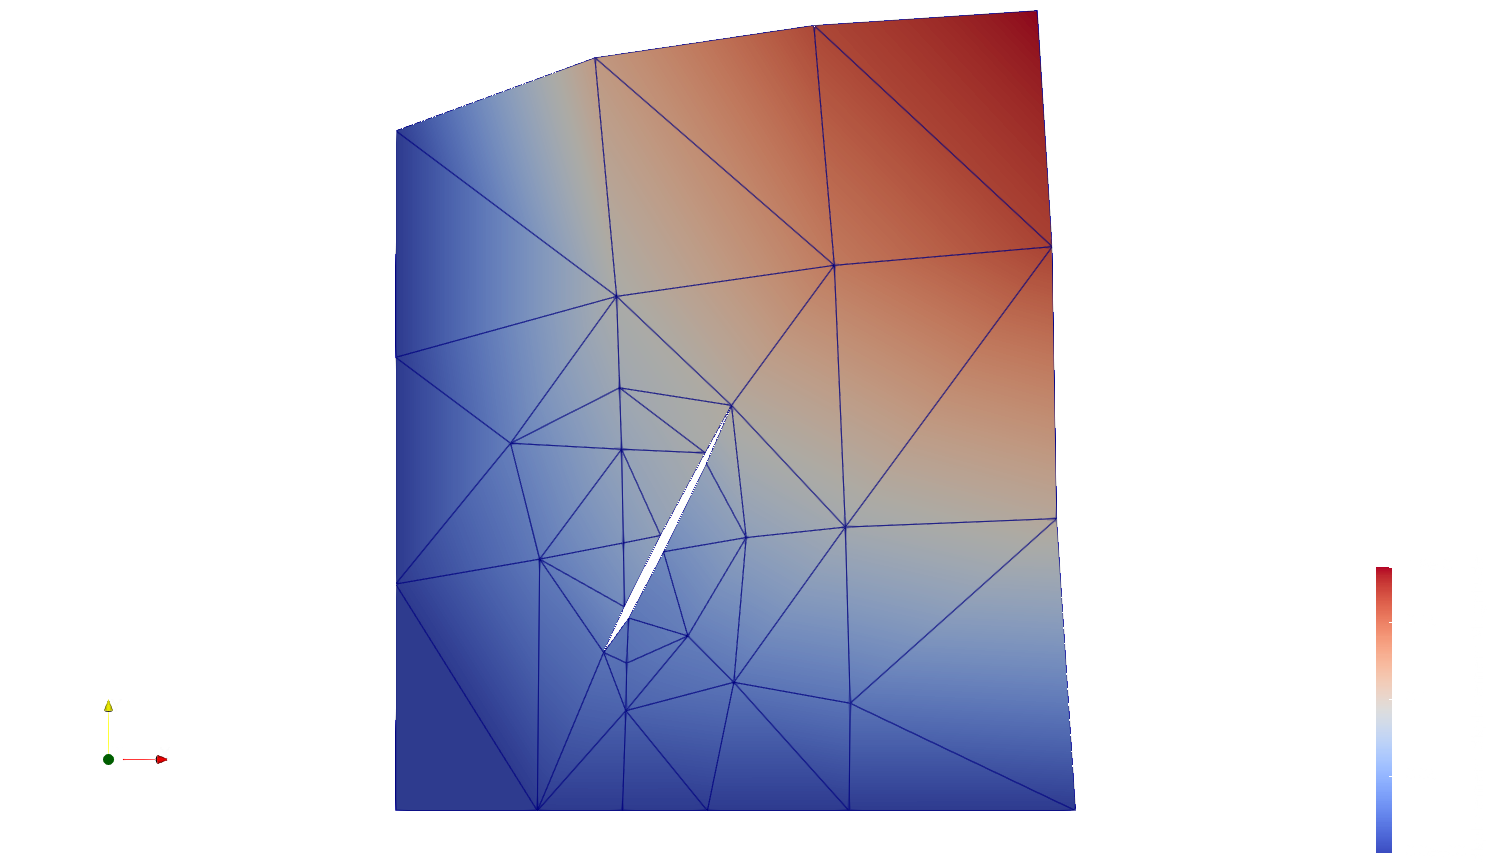
\includegraphics[width=0.6\textwidth]{graphics/ugn_permon_pull.png}
    \caption{}
    \label{fig:ugn_pull}
\end{figure}

V rámci vývoje knihovny PERMON byl implementován generátor problémů lineární
elasticity s puklinami. Funkčnost je prozatím omezena na 2D úlohy. K
implementaci generátoru je využita knihovna PETSc. Konečněprvková síť a
práce na ní je implementována pomocí třídy DMPlex pro práci s
nestrukturovanýmí sítěmi. Díky tomu je mimo jiné možné načítat sítě z
několika formátů (např. Gmsh, ExodusII) a naopak ukládat výsledky do
formátů jako VTK pro následnou vizualizaci. Pukliny implikují podmínky
nepronikání, které jsou implementovány jako lineární nerovnostní
omezení. Vzniklá úloha kvadratického programování je za pomoci knihovny
PERMON dualizována a vyřešena algoritmem MPRGP. 
Výsledek řešení testovací úlohy je na obrázku \ref{fig:ugn_pull}.

% \sy{ÚGN tým se také věnoval vývoji experimentálních kódů v Matlabu na řešení nelineárních hydro-mechanických problémů s puklinami, a to v úzké souvislosti s aktivitami popsanými v následujících dvou kapitolách. Uvažované modely a metody budou popsány níže. Při implementaci byly mimo jiné použity algoritmy dostupné v knihovně PERMON.}

\section{ Matematické modely EDZ a související inverzní úlohy}
\label{sec:hm_modely}
 {\it Období aktivity:}  1/2020 - 6/2021
\subsection{Popis aktivity dle přihlášky projektu}
{\it 
Hlavní náplní aktivity bude testování modelů hydro-mechanických procesů v EDZ se zahrnutím vlivu puklin různých škál. K testování budou využita zejména data z Task G projektu Decovalex (experiment TAS04 v ASPO) případně též dostupná data z podzemní
laboratoře Bukov. Mechanické a hydraulické vlastnosti EDZ budou nejprve odhadnuty pomocí výpočtu napětí v EDZ a použitím modelů poškození. Bude též studován vztah mezi napětím a statistikami mikro puklin. Následně budou uvažovány jednak kontinuální poroelastické modely založené na duální pórovitosti a dále modely založené na kombinaci ekvivalentního porézního média a diskrétní puklinové sítě. Pro různě komplexní modely budou řešeny inverzní úlohy jak pomocí klasických optimalizačních metod tak pomocí
Bayesovského přístupu, který popisuje hledané parametry pomocí statistického rozdělení pravděpodobnosti. Tento přístup vyžaduje výpočetně velmi náročné metody, je však robustnější a přináší více informací(např. kvalitu odhadu hledaných parametrů).}

\subsection{Upřesnění plánu řešení}
Tato aktivita představuje koncepčně nejnáročnější část projektu. Na základě rešerše v rámci aktivity \ref{sec:indikatory} 
a po diskuzi v řešitelském týmu navrhujeme drobné změny a upřesnění postupu z přihlášky. Zaměřili bychom se na reprodukci a rozšíření 
hydro-mechanického modelu a inverzních úloh řešených v rámci projektu DECOVALEX-THMC project (2004–2007), Task A, viz. \cite{Rutqvist2009}. 
V první fázi by šlo o zvládnutí jednoduchého modelu s využitím empirických konstitučních vztahů a založeného na existujících řešičích. 
Rychlé zvládnutí jednoduchého dopředného modelu umožní testování metod Bayesovské inverze. Metamodely, sloužící k urychlení 
výpočtu, lze pak využít k posouzení citlivosti měření na jednotlivé parametry modelu. Jednoduchý dopředný model lze následně nahradit 
víceškálovým modelem, jehož rozvoj závisí na zvládnutí nelinearit na puklinách a nástrojích pro generování regulárních sítí pro náhodné pukliny.  
Paralelně by probíhal vývoj robustnějšího simulačního nástroje v rámci Flow123d,
který by zvládl i výpočet 3d úloh se zahrnutím heterogenity nebo složitějších experimentálních uspořádání.

\subsection{Nelineární hydro-mechanické modely (ÚGN)}
V souladu s popisem této aktivity se ÚGN tým věnoval vývoji nelineárních hydro-mechanických modelů s puklinami, jejich implementací a kombinací s Bayesovskou inverzní analýzou, viz \cite{blaheta2020bayesian}. Konkrétně byly uvažovány dva typy nelinearit: podmínky nepronikání na trhlinách a nelineární závislost hydraulické vodivosti na rozevření trhlin. Podmínka nepronikání byla iteračně řešena pomocí Lagrangeových multiplikátorů, duality a pomocí metody rozkladu oblasti. Druhý typ nelinearity byl linearizován na základě Picardova iteračního schématu. Bayesovská inverzní analýza byla provedena za účelem identifikace neznámých parametrů trhlin a její detailní popis lze najít v následující kapitole. V navazujících publikacích \cite{berevs2021numerical, BBDHH2020} byl popsán další rozvoj těchto modelů a metod.

Dále byl připraven interní dokument "S. Sysala: Investigation of tunnel EDZ by perfect plasticity and mesh
adaptivity", ve kterém byly studovány možnosti mechanického modelování EDZ ve 2D pomocí perfektní plasticity, limitní analýzy zatížení a adaptivity konečněprvkové sítě. Konkrétně bylo zvoleno Drucker-Pragerovo plastické kritérium a dva různé profily tunelů. Ačkoliv limitní parametr zatížení je výrazně vyšší než jedna, odpovídající zóny poškození by mohly určovat směr možného šíření trhlin způsobených ražbou tunelů nebo vrtů.

\section{Knihovny pro stochastické přímé a inverzní metody}
\label{sec:stochastic}
{\it Období aktivity:}  07/2019 - 12/2021

\subsection{Popis aktivity dle přihlášky projektu}
{\it 
Aktivita je zaměřena na vývoj a aplikaci stochastických metod v úlohách simulujících hydro-mechanické procesy v EDZ. V první fázi
bude formulován stochastický popis parametrů uvažovaných modelů včetně popisu rozdělení puklin. Následovat bude implementace
víceúrovňové metody Monte-Carlo (MLMC) se zahrnutím různě detailního popisu puklinových sítí. Bude vyvinut nástroj pro tvorbu
statisticky generovaných puklin a příslušných smíšených výpočetních sítí. Současně budou implementovány specifické metody pro
Bayesovské inverze s využitím metody Metropolis-Hastings pro generování Markovského řetězce. Pro podstatné zvýšení efektivity se
využije přibližný, náhradní (surrogate) model a příslušná varianta Metropolis-Hastings algoritmu (algoritmus se zpožděním).}


\subsection{Víceúrovňová metoda Monte Carlo a výpočty na puklinách (TUL)}

Víceúrovňová metoda Monte Carlo představuje velmi efektivní metodu pro odhad střední hodnoty náhodné veličiny $X$, která je výsledkem 
numerické aproximace. Je využita hierarchie aproximací, kde s klesající přesností aproximace musí výrazně klesat čas výpočtu. 
Pro výpočty metodou konečných prvků lze obvykle získat vhodné aproximace použitím hrubších výpočetních sítí to však není přímo možné
pro smíšené sítě zahrnující diskrétní reprezentaci puklin. Nelze vygenerovat hrubší síť bez odstranění puklin. Za tímto 
účelem byl vyvinut postup nahrazení puklin pomocí heterogenního anisotropního kontinua. V letošním roce byla testovány statistické vlastnosti
rozdílu mezi výpočtem na jemné síti s puklinami a výpočtem na hrubé síti s náhradou pomocí heterogenního kontinua. Pro případ 2d úlohy proudění 
bylo ověřeno, že lze takto získat dobrou aproximaci. Otestování celé víceúrovňové metody na puklinových sítích bude pokračovat v dalším roce.

\begin{figure}
    \centering
    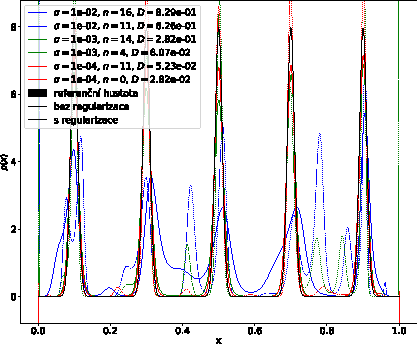
\includegraphics[width=0.6\textwidth]{graphics/five_fingers_regul.pdf}
    \caption{Rekonstrukce hustoty pravděpodobnosti bez regularizace a s jejím použitím pro různé úrovně přesnosti odhadu momentů. Pro méně přesné momenty lze pozorovat výrazné omezení nežádoucích oscilací při použití regularizace.}
    \label{fig:hustota_regul}
\end{figure}


Metoda MLMC umožňuje pouze odhad střední hodnoty, pro bezpečnostní analýzy je však vhodné znát spíše kvantily indikátorů bezpečnosti.
Za tímto účelem rozvíjíme metodu rekonstrukce hustoty pravděpodobnosti pomocí metody maximální entropie. V letošním roce byla vyvinuta 
regularizační technika, která omezuje výskyt nežádoucích oscilací při nedostatečné přesnosti odhadu momentů. Na obrázku 
\ref{fig:hustota_regul} je demonstrován pozitivní efekt na testovacím rozdělení. Dále byla otestována rekonstrukce hustoty pro bivarietní náhodné veličiny.

V rámci paralelně řešeného projektu TAČR (GeoPax) byla dokončena první robustní verze knihovny pro MLMC v příštím roce předpokládáme vyladění technik regularizace a podpory bivarietních rozdělení a začlenění do produkční verze knihovny. Uvedené techniky budou také otestovány na 
úlohách pro predikci indikátorů bezpečnosti.

\subsection{Bayesovské inverzní metody (ÚGN)}

Bayesovská inverze je přirozeným nástrojem pro odhad neznámých parametrů matematického modelu na základě odezvy modelu zatížené nejistotami způsobenými například chybami měření. V roce 2020 tým ÚGN pokračoval ve vývoji metod pro efektivní numerickou realizaci Bayesovské inverze. Numerická realizace spočívá v generování snímků  z aposteriorního rozdělení neznámých parametrů, což vyžaduje vysoký počet vyhodnocení modelu. Pro zvýšení efektivity používáme algoritmus Metropolis-Hastings se zpožděným přijetím (DAMH), ve kterém jsou některá vyhodnocení modelu nahrazena vyhodnocením výpočetně levnějšího zástupného modelu ({\it eng. surrogate model}). V případě velmi vysoké výpočetní náročnosti matematického modelu je rovněž možné přejít k plnému nahrazení zástupným modelem.

Hlavním výsledkem je vývoj a implementace zástupných modelů, které lze využít v přímých i inverzních úlohách s nejistotami. Mimo jiné jsme implementovali polynomiální zástupný model, který je v průběhu DAMH algoritmu dále zpřesňován pomocí nově získaných vyhodnocení původního modelu. Model je neintruzivní a tedy široce využitelný. Při využití snímků ke zpřesňování modelu se nabízí více strategií, které budou dále testovány.

Popsaný přístup byl aplikován na vybrané hydro-mechanické úlohy, byl proveden odhad hydraulické vodivosti a parametrů trhliny na základě nepřesných měření toku na hranici oblasti, viz \cite{blaheta2020bayesian, BBDHH2020, berevs2021numerical}. Dále byly navrženy inverzní úlohy, které je možné řešit v rámci analýzy propustnosti EDZ, viz \cite{domesova2021efficient}. Další vývoj v této oblasti je očekáván i v roce 2021.

ÚGN tým se navíc věnoval efektivní implementací stochastické Galerkinovy metody, která slouží k řešení  lineárních úloh s nejistotami a lze rovněž využít jako zástupný model, viz \cite{berevs2020comparison}.


% \bigskip
% \sy{Honzo, předpokládám, že níže uvedené popisy publikací jsou pro Tvou potřebu. Kdybys to ale chtěl nechat ve zprávě, nemám s tím problém. Jinak výše uvedený text od Simony jsem trochu poupravil a přeuspořádal.}

\vspace{2ex}
% \noindent{\it Publikované články:}

% \noindent

% \cite{BBDHH2020} - Příspěvek se věnuje řešení inverzních úloh identifikace materiálových parametrů hornin (např. hydraulické vodivosti). Je uvažován porézní materiál s trhlinami, které mohou být zahrnuty v~kontinuálním modelu, nebo modelovány explicitně. Jsou navrženy dva přístupy k analýze propustnosti EDZ. Dále je porovnáno použití deterministických a stochastických metod. Stochastický (Baysovský) přístup je robustnější, poskytuje více informací o neznámých parametrech, ale je výpočetně velice náročný, vyžaduje tedy další výzkum v oblasti efektivní numerické realizace.

% \vspace{2ex}
% \noindent
% \cite{berevs2020comparison} - Stochastická Galerkinova metoda umožňuje řešení lineárních úloh s nejistotami v parametrech v rámci monolitické soustavy lineárních rovnic v tenzorovém formátu. Článek se zabývá efektivní implementací stochastické Galerkinovy metody, porovnává několik přístupů ke konstrukci redukované báze. Tento přístup přirozeně slouží k řešení přímých úloh s nejistotami a také může být použit jako zástupný model pro Bayesovskou inverzi.

% \vspace{2ex}
% \noindent
% \cite{domesova2021efficient} - Příspěvek je zaměřen na využití neintruzivních zástupných modelů ke zvýšení efektivity Markov chain Monte Carlo metod. Výsledkem je proces generování vzorků z aposteriorního rozdělení, který má díky neintruzivnímu charakteru obecné využití. Zde byl přístup aplikován na dvě modelové úlohy hydromechaniky (odhad hydraulické vodivosti, odhad rozevření trhliny).

% \vspace{2ex}
% \noindent
% \cite{berevs2021numerical} - M. Béreš, R. Blaheta, S. Domesová, D. Horák. Numerical methods for simulation of coupled hydro-mechanical processes in fractured porous media. Proceedings of IACMAG 2020. LNCE 125, Springer (přijato)

% Témata, kterým se věnuje ÚGN (vývoj hydro-mechanického modelu s kontakty v trhlinách a Bayesovské inverzní metody) spolu úzce souvisí. Tento příspěvek je zaměřen na numerické řešení hydro-mechanických úloh v porézním prostředí s trhlinami modelovanými explicitně. Hlavním výsledkem je zajištění podmínky nepronikání a řešení kontaktu v trhlinách pomocí Lagrangeových multiplikátorů. Dále jsme pokročili ve vývoji iteračních metod pro řešení výsledných sdružených úloh. Výsledný model slouží jako aplikační úloha pro Bayesovskou inverzi.



\section{Modely transportu (TUL)}
\label{sec:transport}

Jelikož se pozdrželo plánování aktivity \ref{sec:hm_modely}, byl zatím týmem TUL s předstihem realizován model proudění a transportu, 
viz. příloha \uv{model\_transportu.pdf}, který byl plánován jako součást aktivity "Vývoj specializovaného nástroje pro predikci indikátorů bezpečnosti" začínající v roce 2021. Model zahrnující stacionární proudění a transport konzervativního stopovače s difúzí a disperzí je realizován simulátorem Flow123d a bude sloužit k vlastnímu výpočtu indikátorů bezpečnosti. Celý model včetně procedurálně generované geometrie a výpočetní sítě je parametrizován a umožní tak jednak snadnou úpravu s ohledem na konkrétní 
lokalitu, tak stochastické výpočty nebo inverzní úlohy pro použité parametry.

Na základě realizovaných výpočtu byly identifikovány následující problémy, které je třeba dále řešit:
\begin{itemize}
    \item Program GMSH použitý pro přípravu geometrie a výpočetní sítě má problémy s tvorbou sítě pro větší počet puklin, nebo v případě složitějších průniků s geometrií chodeb. Zdá se, že pro řešení problému je třeba najít způsob jak přesněji definovat 
    krok sítě, tak abychom dosáhli adaptivního zjemnění pouze v okolí chodeb a jejich průsečíků s vrty.
    \item EDZ je popsána pouze jednou vrstvou elementů o tloušťce 2m. Je třeba zvládnou přesnější popis EDZ aniž by došlo k výraznému nárůstu počtu elementů. Bude snaha využít anisotropních elementů pro zjemnění pouze ve směru kolmém na stěnu chodeb.
    \item Při použití větších časových kroků vykazuje použité DG výpočetní schéma transportu výrazné oscilace. Tomu snad lze zabránit
    pečlivější volbou regularizačního parametru, nebo použitím metody vyššího řádu.
    \item Pro účely vyhodnocení indikátorů bude třeba simulátor Flow123d doplnit o výstup některých hodnot na hranici oblasti.
\end{itemize}

\subsection{Analytický transport}
Bylo implementováno analytické řešení advekčně-difúzní rovnice v 1D.  
Řešení postihuje procesy advekce, difúze a lineární sorpce. Řešení rovněž umožňuje zahrnout rozpadový člen a ředění.

Výpočet byl implementován v jazyce Python. Výsledná třída umožňuje pro zadané parametry konstrukci konvolučního jádra, 
které je pak možno aplikovat pro různý průběh koncentrace na vtokové hranici modelové domény. 

Výstupy SW byly na zvolené testovací úloze ověřeny proti výstupům simulátoru Flow123d. 
Testovací úlohy byly počítány s parametry uvedenými v Tabulce \ref{parametry}, kde Kd je distribuční koeficient lineární sorpce, 
L je délka modelové domény, Rho je hustota a T je simulační perioda. Byly spočteny 4 varianty sad hodnot rychlosti a efektivní difuzivity (viz Tabulka \ref{varianty}). Analytické řešení výpočet pro nulovou difúzi (vedlo na dělení nulou), ve variantě v0 je proto počítáno s hodnotou 0,01.

Výsledky všech variant testovací úlohy jsou znázorněny na Obrázku \ref{results}. 
Z výsledků je patrná relativně dobrá shoda. Pro úlohy s převažující advekcí se silně ve výsledcích Flow123d silně projevuje 
numerická difúze.

\begin{table}[ht]
\begin{center}
    \caption{Varianty modelu 1D transportu.}
    \begin{tabular}{ | l | c | c | c | c |}
    \hline
    \small  & \small v0 & \small v1 & \small v2 & \small v3\\ \hline
    \small rychlost [$\rm m*s^{-1}$] & \small 10 & \small 10 & \small 10 & \small 10\\ \hline
    \small De [$\rm m^{2}*s^{-1}$] & \small 0 & \small 1 & \small 10 & \small 100\\ \hline
    \end{tabular}
    \label{varianty}
\end{center}
\end{table}

\begin{table}[ht]
\begin{center}
    \caption{Parametry modelu 1D transportu.}
    \begin{tabular}{ | l | c |}
    \hline
    \small porozita & \small 1\\ \hline
    \small Kd & \small 0 $\rm m^{3}*kg^{-1}$\\ \hline
    \small L & \small 1000 $\rm m$\\ \hline
    \small Rho & \small 2700 $\rm kg*m^{-3}$\\ \hline
    \small T & \small 150 $\rm let$\\ \hline
    \end{tabular}
    \label{parametry}
\end{center}
\end{table}

\begin{figure}[h]
\centering
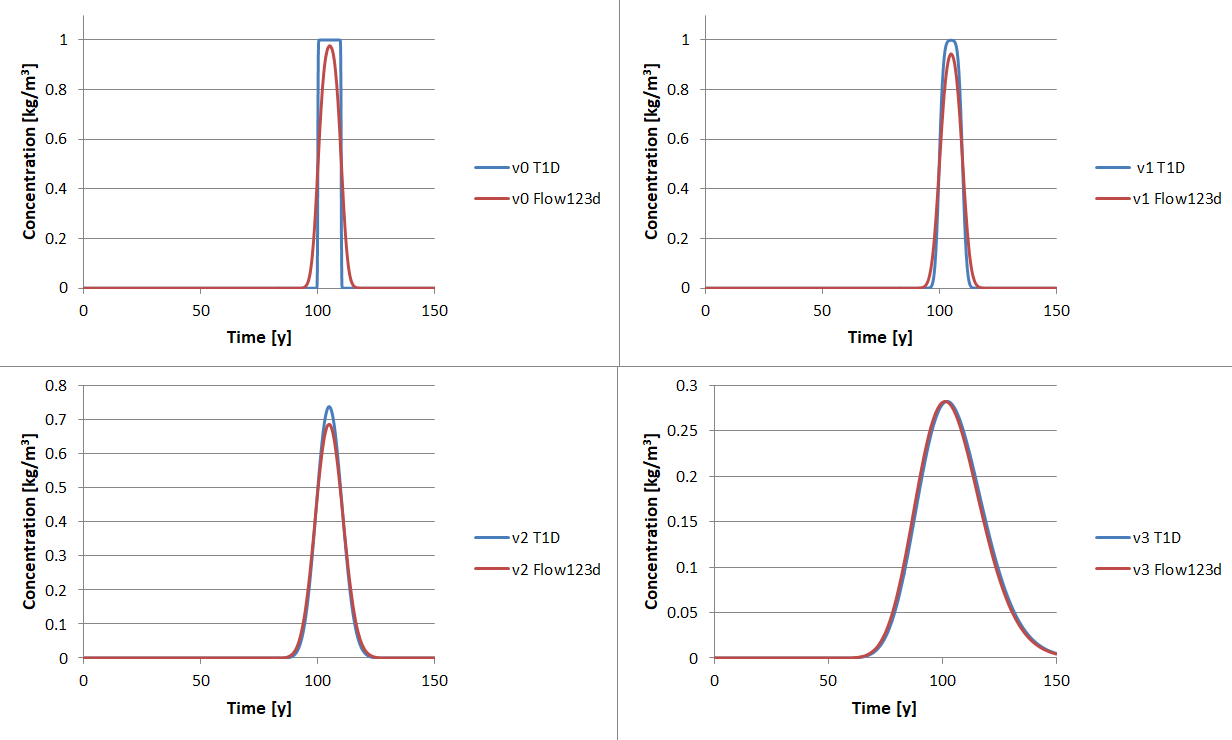
\includegraphics[width=\textwidth]{graphics/v0_3.png}
\caption{Výsledky testovací úlohy 1D transportu - porovnání analytického řešení a Flow123d}
\label{results}
\end{figure}


\section{Závěr}
Během roku 2020 byly realizovány přípravné vývojové práce a byl upřesněn postup dosažení výsledků projektu tak, aby 
vývoj jednotlivých modelů byl pokud možno nezávislý. Za tímto účelem budou nejprve realizovány jednoduché modely založené na existujících kódech, aby bylo možno testovat stochastické výpočty, Bayesovské inverze a integraci celého výpočtu.
Následně budou jednotlivé komponenty iterativně vylepšovány nebo nahrazeny pokročilejším modelem.  Toto se týká zejména 
pokročilých modelů mechaniky a víceškálového modelu pro určení parametrů EDZ.

S ohledem na dosavadní průběh řešení navrhujeme následující změny v harmonogramu projektu:
\begin{itemize}
    \item Aktivita "Vývoj modelu proudění a mechaniky na smíšených sítích", bude pokračovat v roce 2021 s cílem 
zvládnout kontakty, tření a rozevírání puklin. Bude otestován přístup, kdy jsou tyto jevy modelovány pomocí 
nelineární závislosti mezi tenzorem napětí a deformace. Tento přístup se jeví jako fyzikálně relevantnější a z praktického 
hlediska umožňuje značnou flexibilitu ve volbě konkrétního konstitutivního vztahu. Do konce roku 2021 bude tento přístup ověřen
a pokud se osvědčí bude možno v rámci projektu realizovat víceškálový model EDZ.
    \item Aktivita "Matematické modely EDZ a související inverzní úlohy" bude prodloužena až do konce roku 2021 s 
    cílem reprodukovat výsledky HM modelů pro data z experimentu TSX (za předpokladu přístupu k datům). Pro co nejjednodušší 
    model bude otestováno použití metod pro Bayesovskou inverzi s cílem získat informaci o rozdělení parametrů modelu. Původně zamýšlené využití dat z experimentu TAS04 v ASPO nebude realizováno, předchozí snahy více týmů postihnout naměřená data byly neúspěšné.  
    \item Realizace aktivity "Predikce indikátorů bezpečnosti" bude validována s využitím dat z experimentu TSX.
\end{itemize}


\bibliographystyle{plain}
%\bibliographystyle{dinat-etal}
\bibliography{zprava.bib}

% \newpage
% \section{Příloha}
% \subsection{Výsledky modelu transportu}

% \subsubsection{Varianta 1}
% \begin{figure}[H]
% \centering
% 
\includegraphics[width=16cm]{graphics/obr_ralek/nek_zdroj/01_3w.png}
% 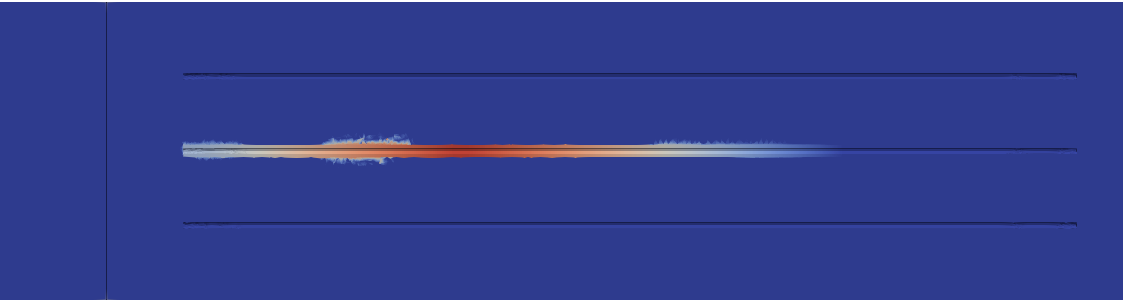
\includegraphics[width=16cm]{graphics/obr_ralek/nek_zdroj/02_4m.png}
% 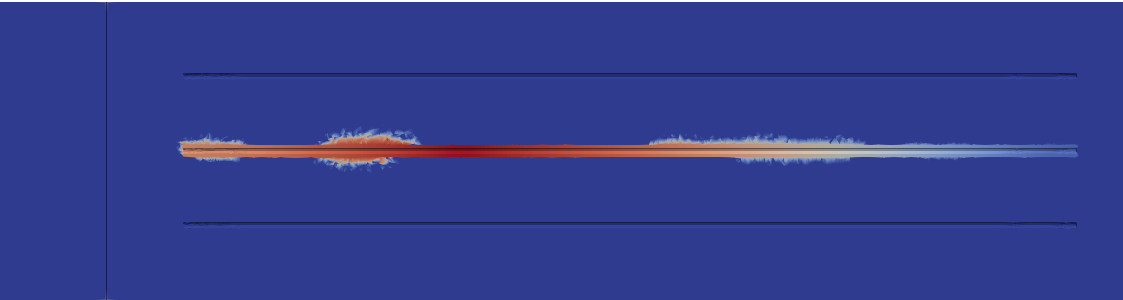
\includegraphics[width=16cm]{graphics/obr_ralek/nek_zdroj/03_1a.png}
% 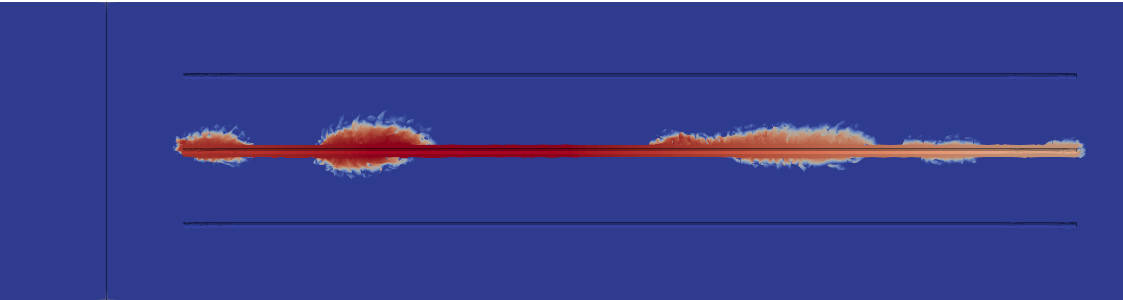
\includegraphics[width=16cm]{graphics/obr_ralek/nek_zdroj/04_3a.png}
% 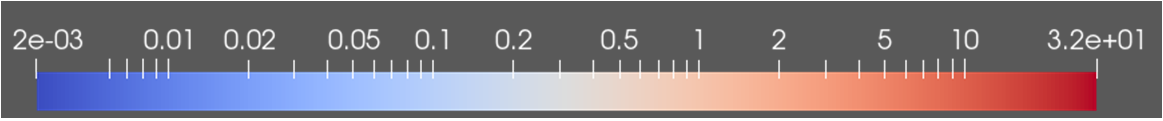
\includegraphics[width=16cm]{graphics/obr_ralek/nek_zdroj/skala_nek_zdroj.png}
% \caption{Prostorové rozložení koncentrace izotopu $^{129}I$ v~různých časech, odshora: 3 týdny, 4 měsíce, 1 rok, 3 roky. Horizontální řez oblastí.}
% \label{nek_zdroj_01}
% \end{figure}

% \begin{figure}[H]
% \centering
% 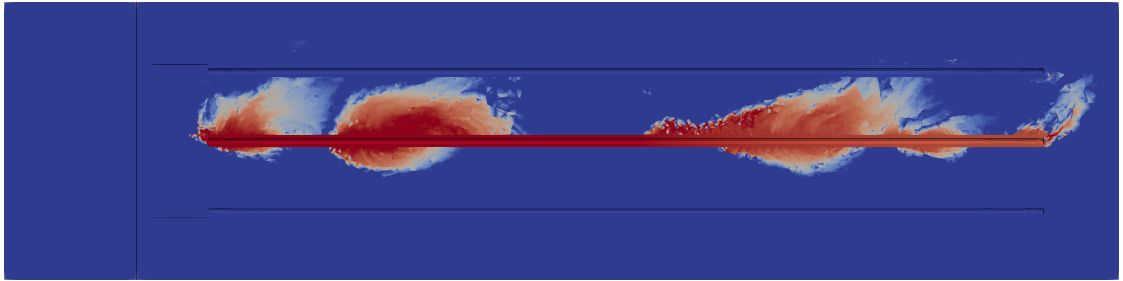
\includegraphics[width=16cm]{graphics/obr_ralek/nek_zdroj/05_6a.png}
% 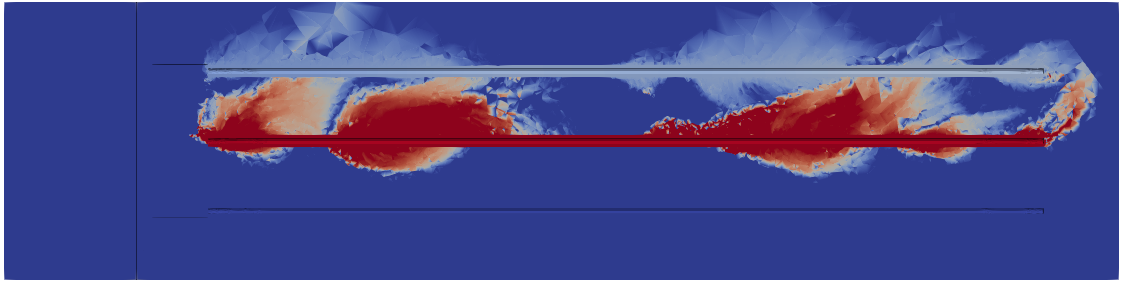
\includegraphics[width=16cm]{graphics/obr_ralek/nek_zdroj/06_20a.png}
% 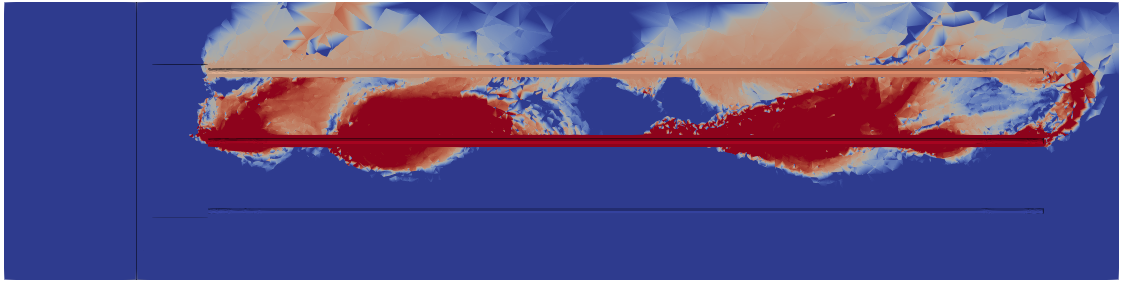
\includegraphics[width=16cm]{graphics/obr_ralek/nek_zdroj/07_50a.png}
% 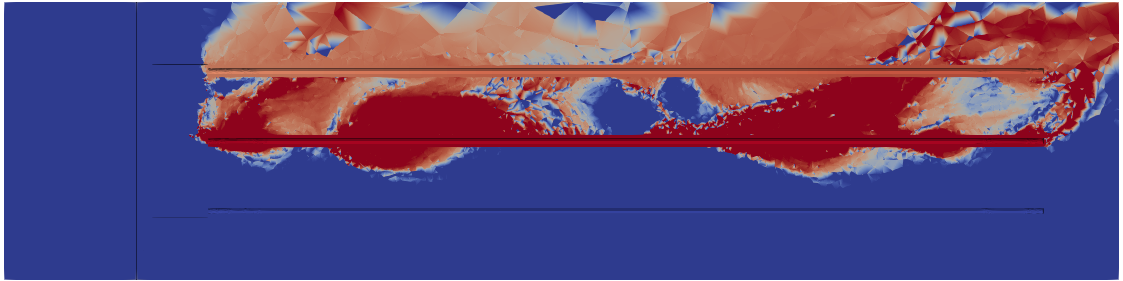
\includegraphics[width=16cm]{graphics/obr_ralek/nek_zdroj/08_300a.png}
% 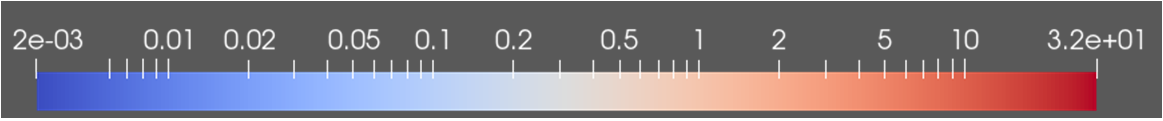
\includegraphics[width=16cm]{graphics/obr_ralek/nek_zdroj/skala_nek_zdroj.png}
% \caption{Prostorové rozložení koncentrace izotopu $^{129}I$ v~různých časech, odshora: 6 let, 20 let, 50 let, 300 let.Horizontální řez oblastí.}
% \label{nek_zdroj_02}
% \end{figure}

% \subsubsection{Varianta 2}
% \begin{figure}[H]
% \centering
% 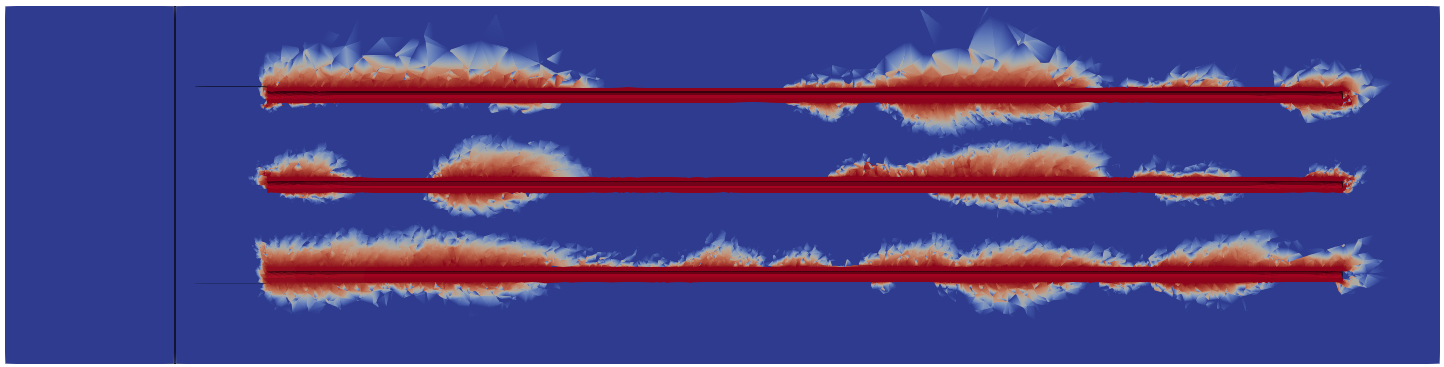
\includegraphics[width=16cm]{graphics/obr_ralek/var2/001a.png}
% 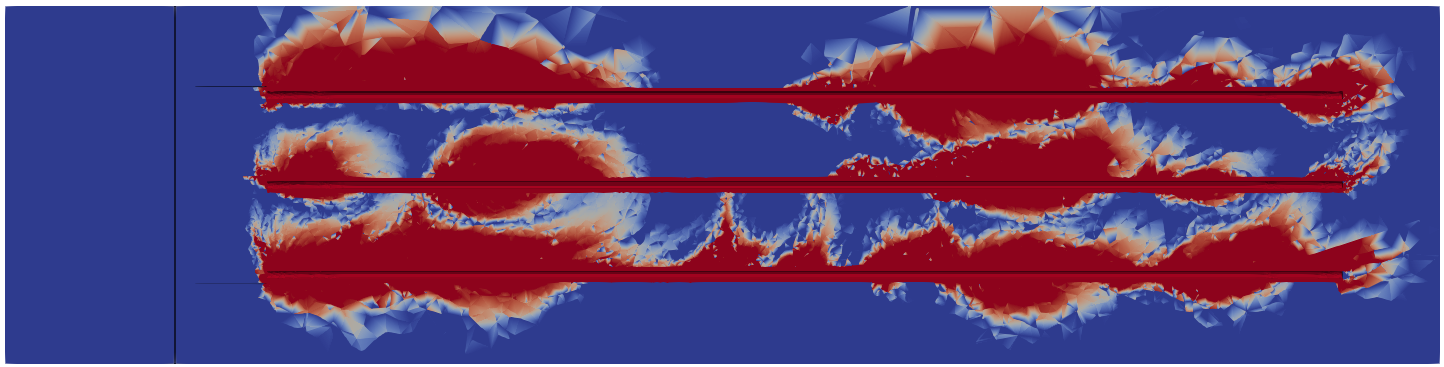
\includegraphics[width=16cm]{graphics/obr_ralek/var2/010a.png}
% 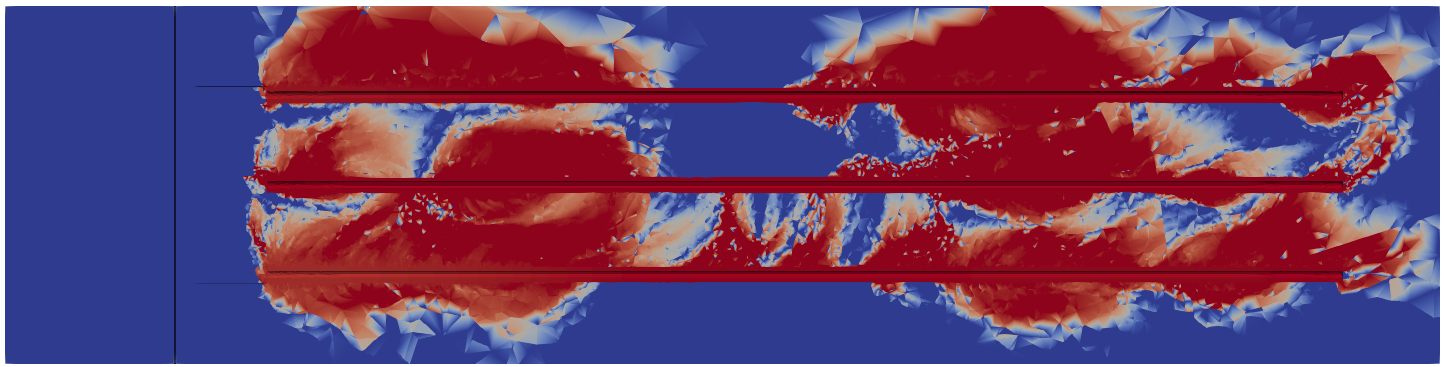
\includegraphics[width=16cm]{graphics/obr_ralek/var2/020a.png}
% 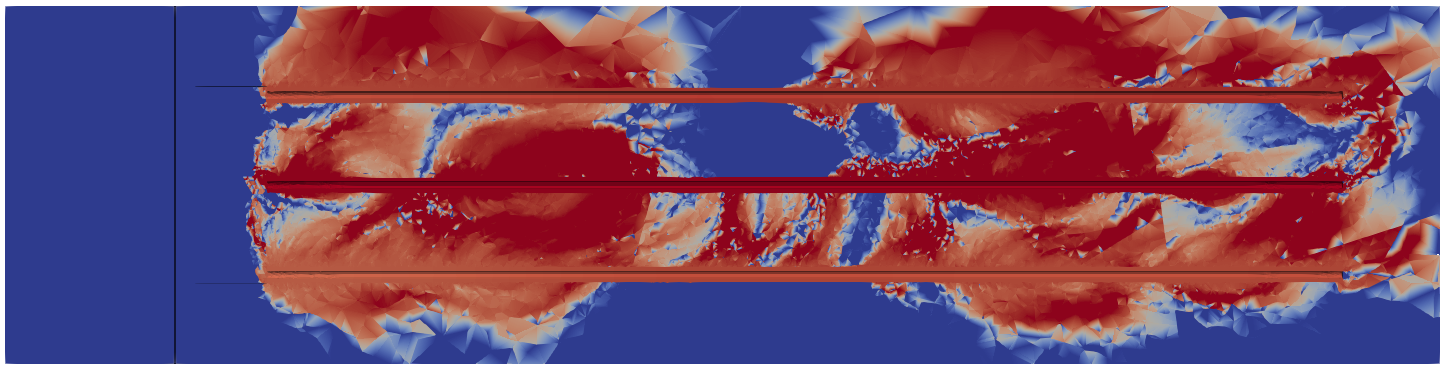
\includegraphics[width=16cm]{graphics/obr_ralek/var2/030a.png}
% 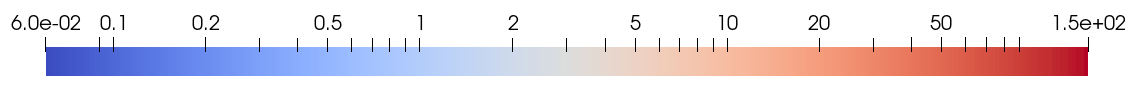
\includegraphics[width=16cm]{graphics/obr_ralek/var2/skala_var2.png}
% \caption{Prostorové rozložení koncentrace izotopu $^{129}I$ v~různých časech, odshora: 1, 10, 20, 30 let. Horizontální řez oblastí.}
% \label{...}
% \end{figure}

% \begin{figure}[H]
% \centering
% 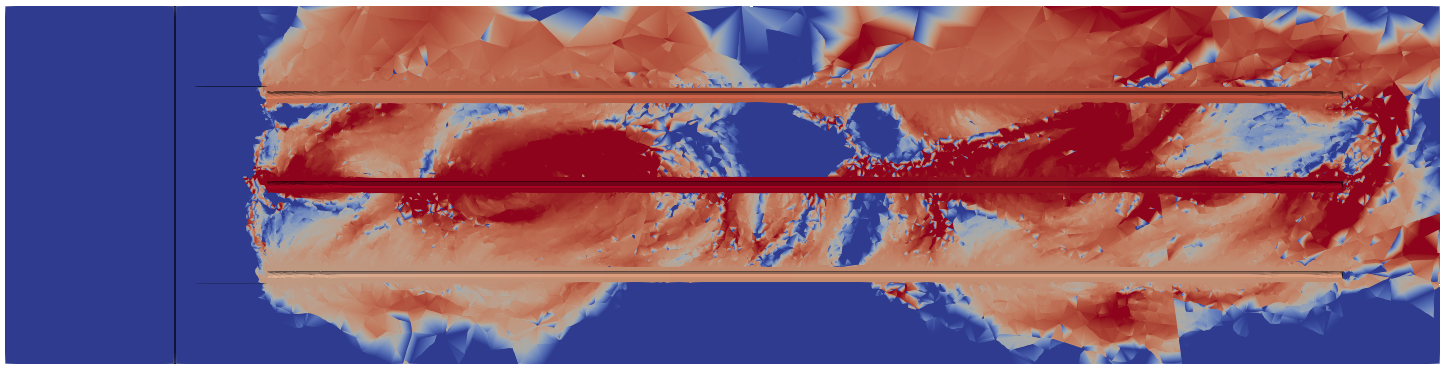
\includegraphics[width=16cm]{graphics/obr_ralek/var2/050a.png}
% 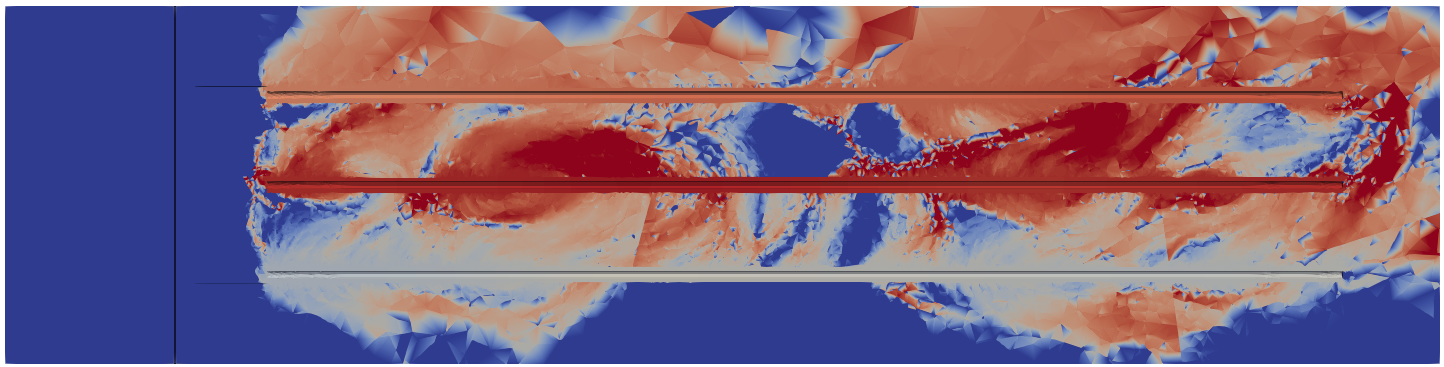
\includegraphics[width=16cm]{graphics/obr_ralek/var2/070.png}
% 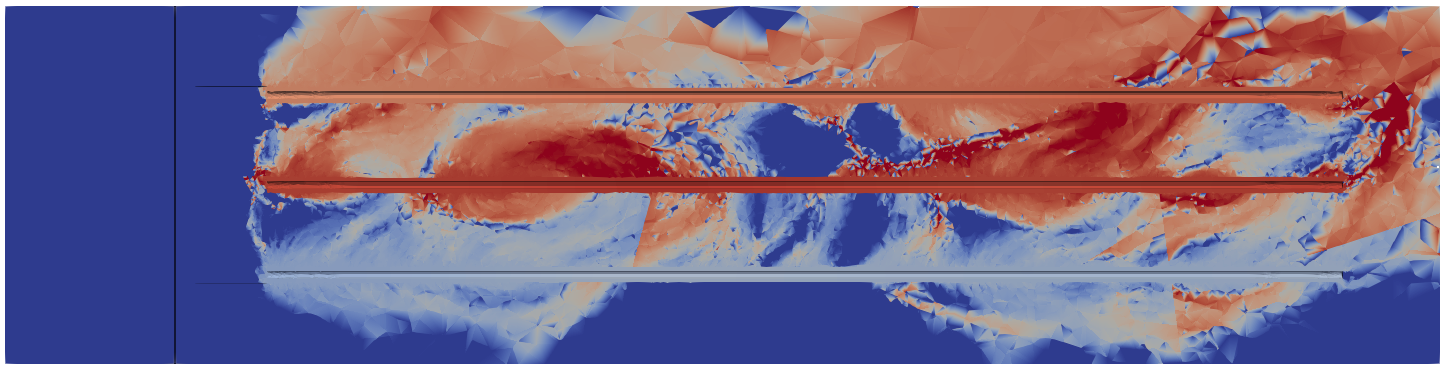
\includegraphics[width=16cm]{graphics/obr_ralek/var2/100a.png}
% 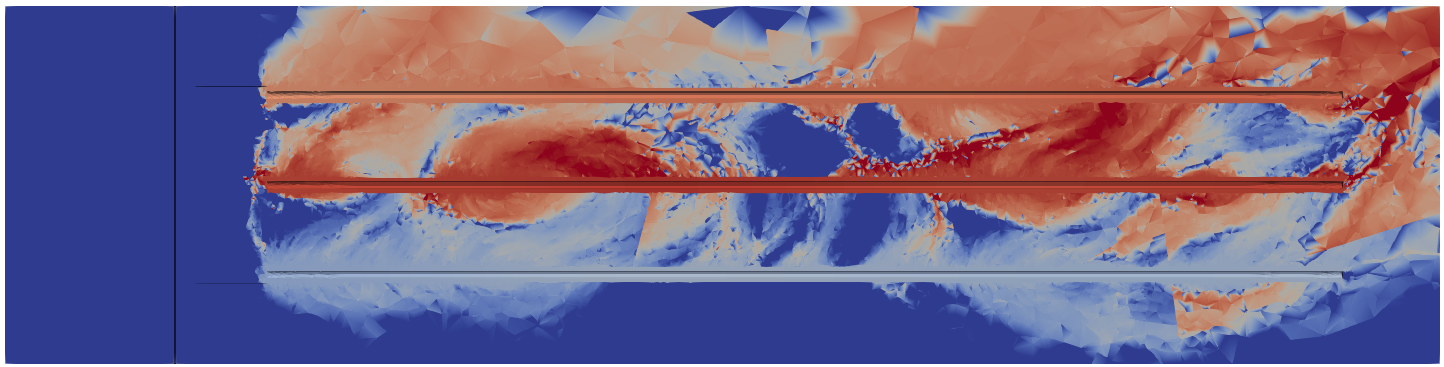
\includegraphics[width=16cm]{graphics/obr_ralek/var2/160a.png}
% 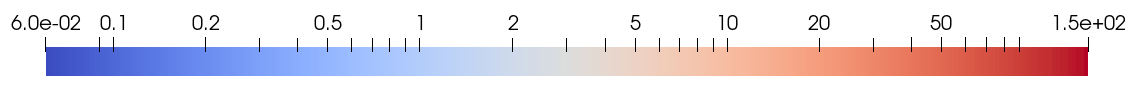
\includegraphics[width=16cm]{graphics/obr_ralek/var2/skala_var2.png}
% \caption{Prostorové rozložení koncentrace izotopu $^{129}I$ v~různých časech, odshora: 50, 70, 100, 160 let. Horizontální řez oblastí.}
% \label{...}
% \end{figure}

% \begin{figure}[H]
% \centering
% 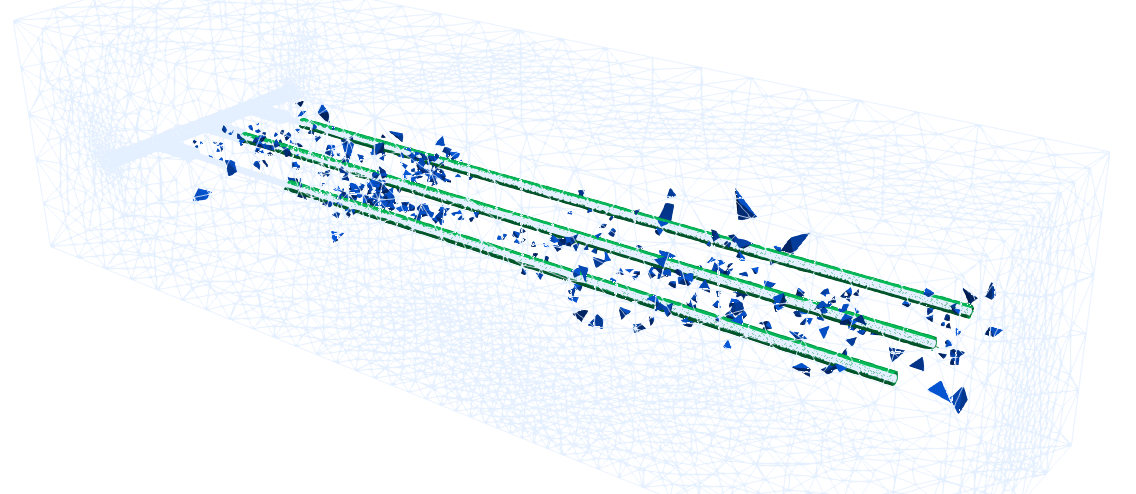
\includegraphics[width=12cm]{graphics/obr_ralek/var2/oscilace/01a.png}
% 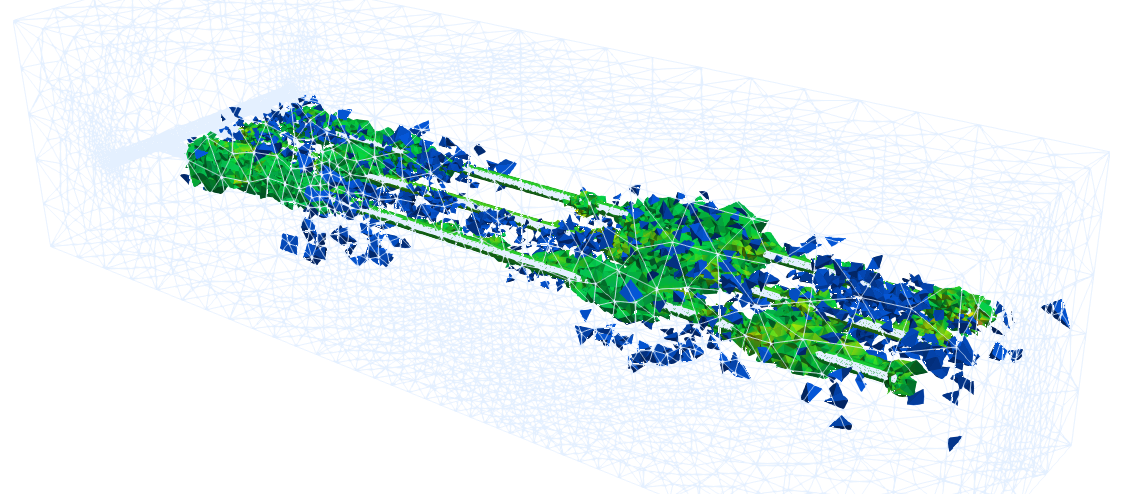
\includegraphics[width=12cm]{graphics/obr_ralek/var2/oscilace/10a.png}
% 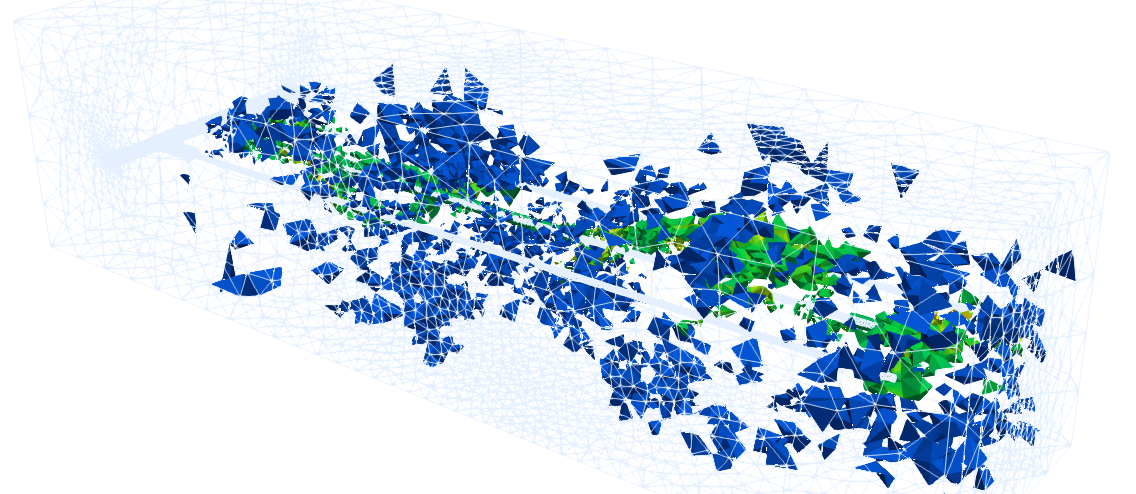
\includegraphics[width=12cm]{graphics/obr_ralek/var2/oscilace/50a.png}
% 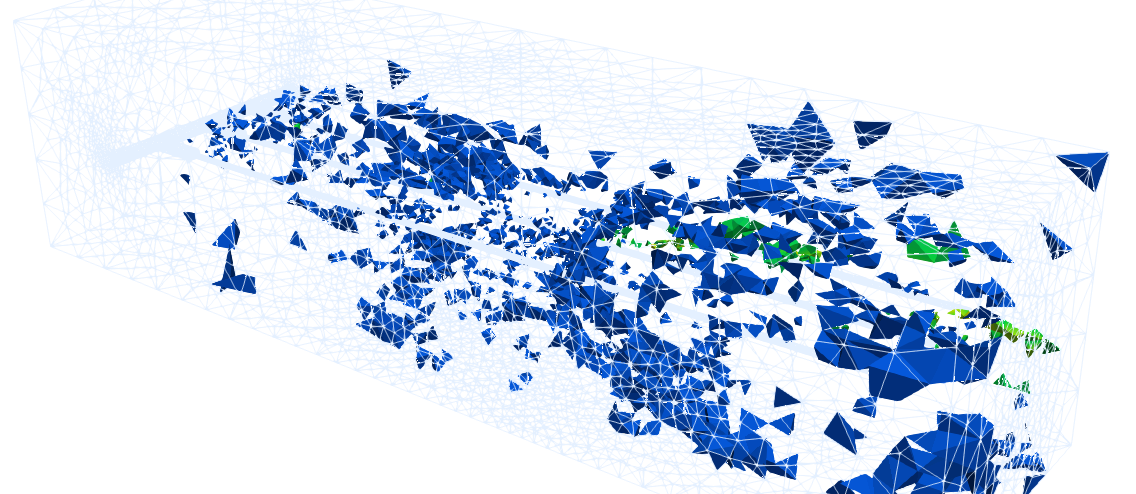
\includegraphics[width=12cm]{graphics/obr_ralek/var2/oscilace/150a.png}
% \caption{numerické oscilace; 1, 10, 50, 150 let}
% \label{oscilace_3D}
% \end{figure}

% \begin{figure}[H]
% \centering
% 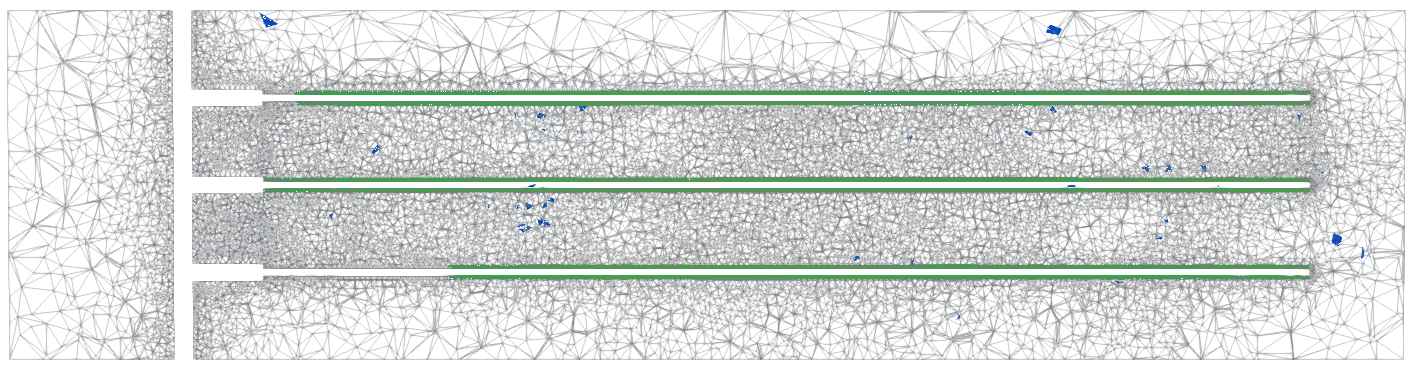
\includegraphics[width=16cm]{graphics/obr_ralek/var2/oscilace/slice01a.png}
% 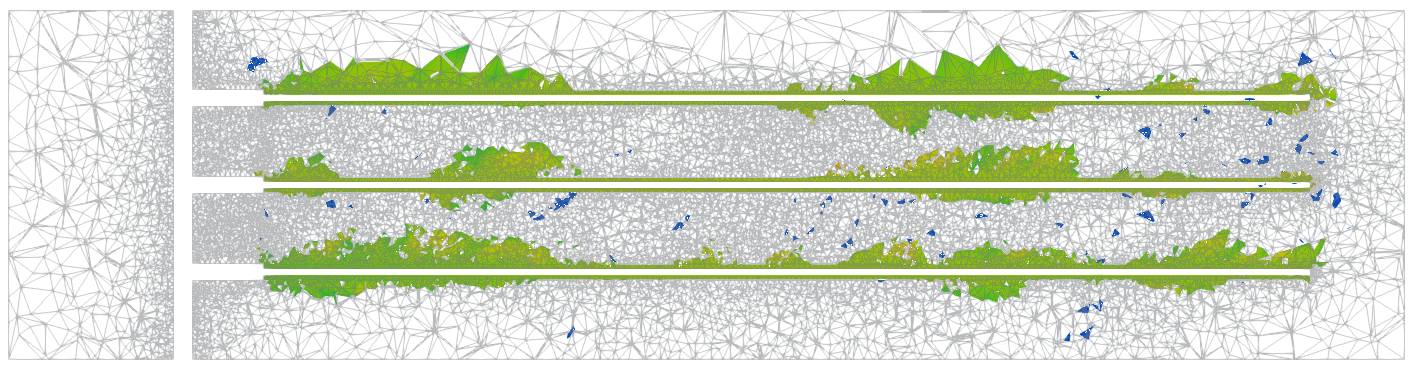
\includegraphics[width=16cm]{graphics/obr_ralek/var2/oscilace/slice10a.png}
% 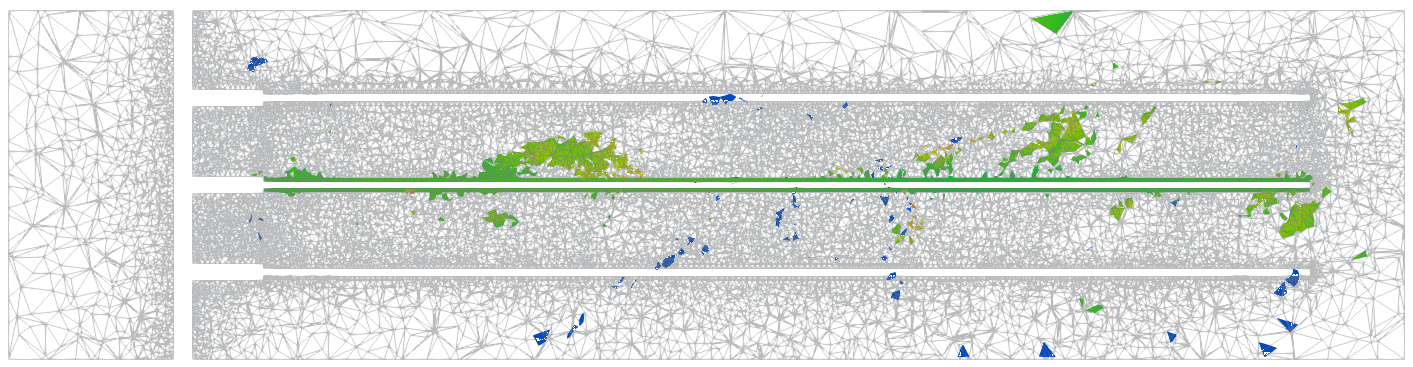
\includegraphics[width=16cm]{graphics/obr_ralek/var2/oscilace/slice40a.png}
% 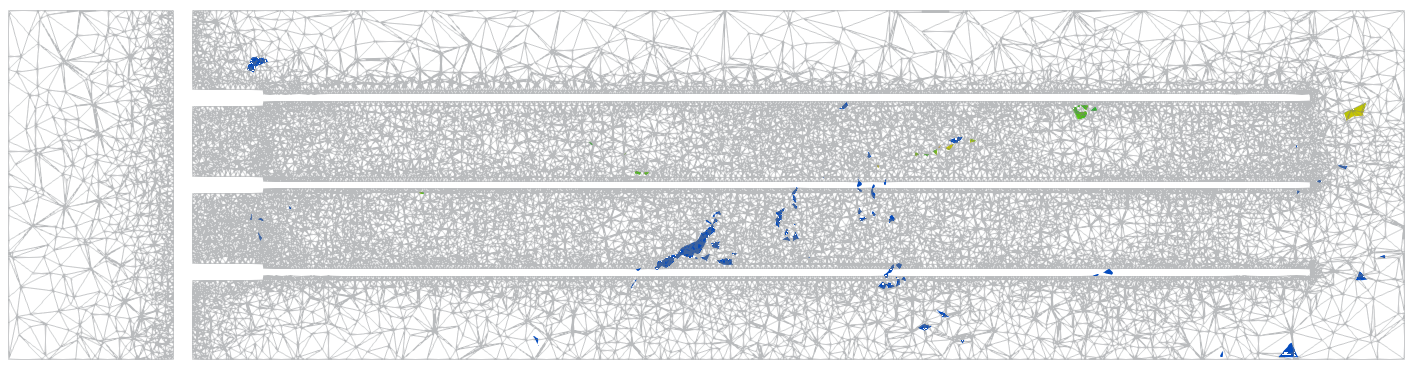
\includegraphics[width=16cm]{graphics/obr_ralek/var2/oscilace/slice150a.png}
% \caption{numerické oscilace; 1, 10, 40, 150 let}
% \label{oscilace_slice}
% \end{figure}

% \subsubsection{Varianta 3}
% \begin{figure}[H]
% \centering
% 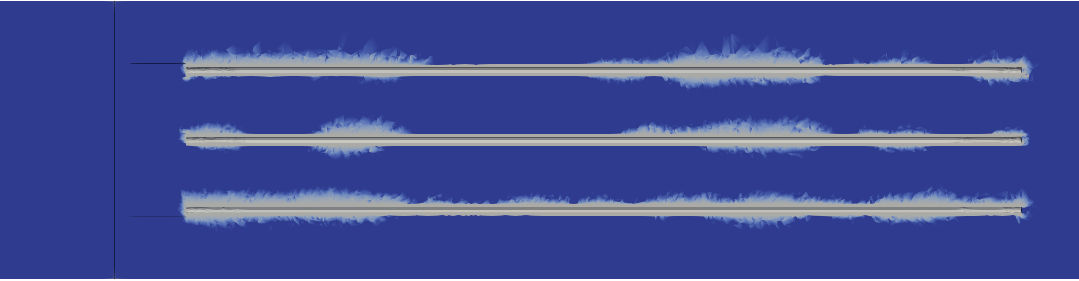
\includegraphics[width=16cm]{graphics/obr_ralek/var3/02_1y.png}
% 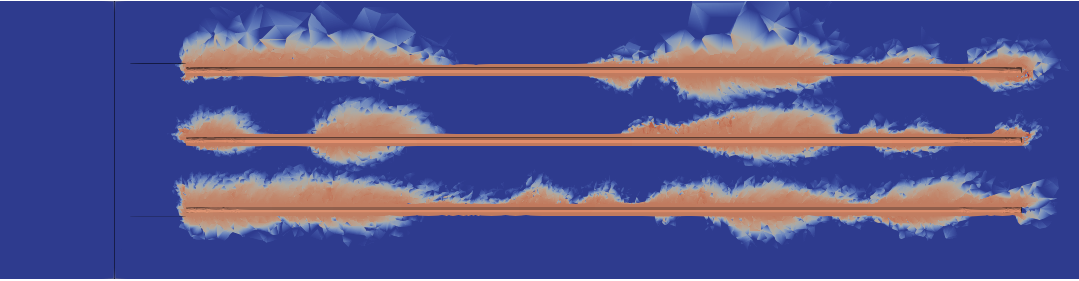
\includegraphics[width=16cm]{graphics/obr_ralek/var3/04_6y.png}
% 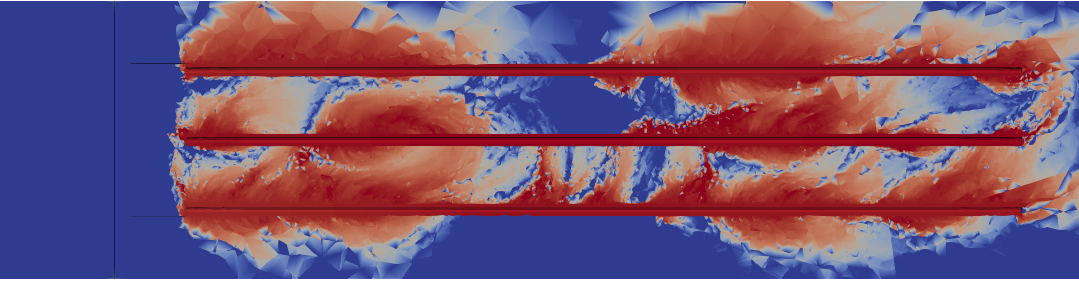
\includegraphics[width=16cm]{graphics/obr_ralek/var3/06_19y.png}
% 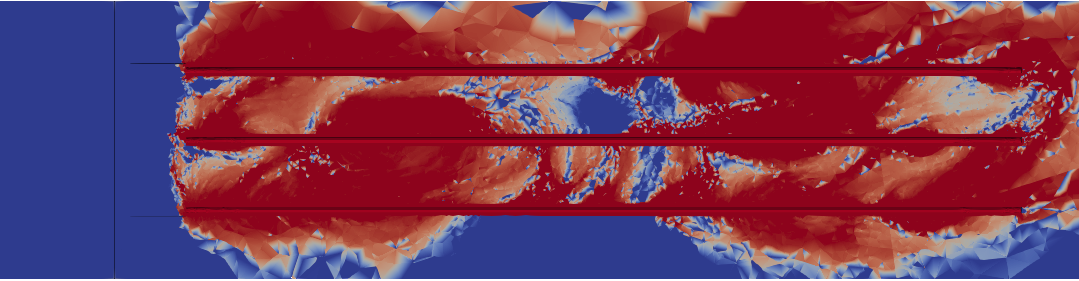
\includegraphics[width=16cm]{graphics/obr_ralek/var3/07_95y.png}
% 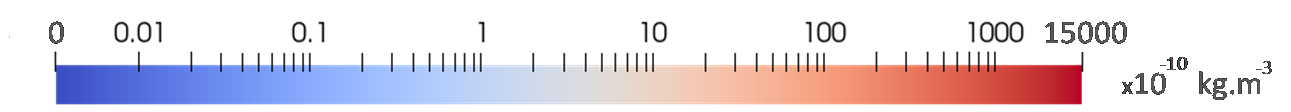
\includegraphics[width=16cm]{graphics/obr_ralek/var3/skala_nek_zdroj_vypnuti.png}
% \caption{Prostorové rozložení koncentrace izotopu $^{129}I$ v~různých časech, odshora: 1 rok, 6 let, 19 let, 95 let. Horizontální řez oblastí.}
% \label{nek_zdroj_vyp_01}
% \end{figure}

% \begin{figure}[H]
% \centering
% 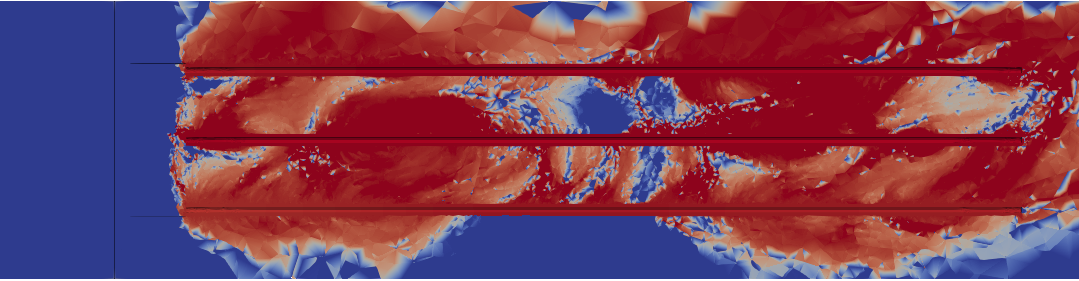
\includegraphics[width=16cm]{graphics/obr_ralek/var3/08_158y.png}
% 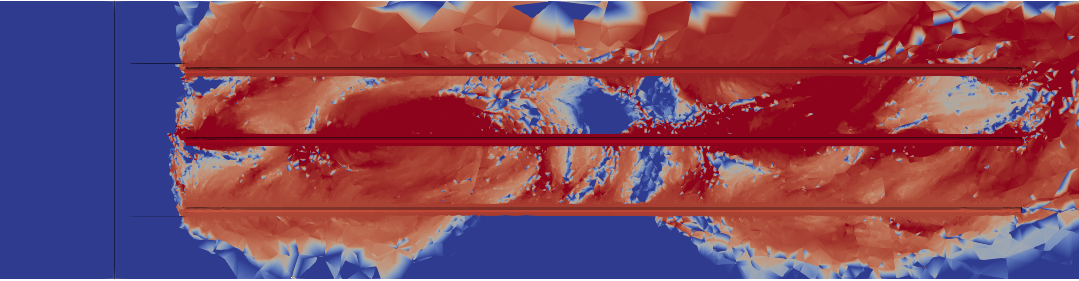
\includegraphics[width=16cm]{graphics/obr_ralek/var3/09_222y.png}
% 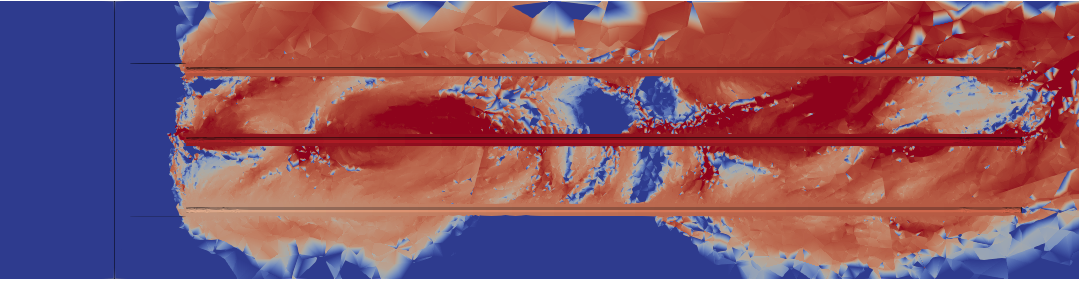
\includegraphics[width=16cm]{graphics/obr_ralek/var3/10_285y.png}
% 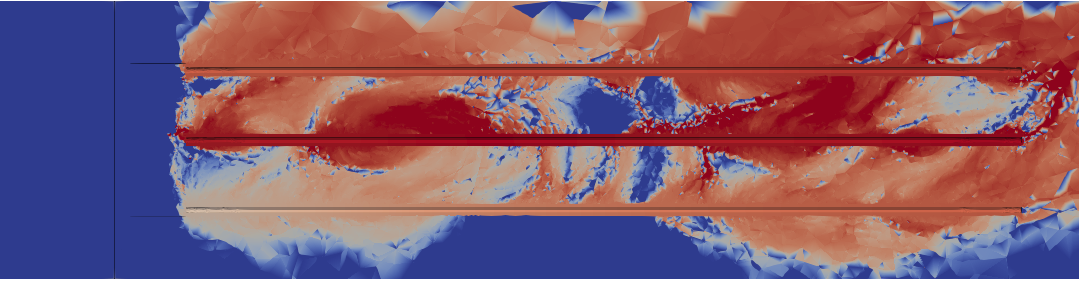
\includegraphics[width=16cm]{graphics/obr_ralek/var3/13_1046y.png}
% 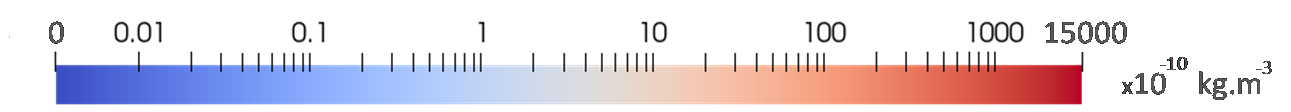
\includegraphics[width=16cm]{graphics/obr_ralek/var3/skala_nek_zdroj_vypnuti.png}
% \caption{Prostorové rozložení koncentrace izotopu $^{129}I$ v~různých časech, odshora: 158 let, 222 let, 285 let, 1046 let.Horizontální řez oblastí.}
% \label{nek_zdroj_vyp_02}
% \end{figure}

\end{onehalfspacing} 

\end{document}
